\documentclass[polish,12pt]{aghthesis}
% \documentclass[english,12pt]{aghthesis} dla pracy w języku angielskim. Uwaga, w przypadku strony tytułowej zmiana języka dotyczy tylko kolejności wersji językowych tytułu pracy. 

% Szablon przystosowany jest do druku dwustronnego. 

\usepackage[latin2]{inputenc}
\usepackage{url}
\usepackage{indentfirst}
\usepackage{graphicx}
\usepackage{float}
\usepackage{listings}
\usepackage{color}
\usepackage{xcolor}
\usepackage{siunitx}
\usepackage{caption}

\renewcommand{\arraystretch}{1.3}
\renewcommand{\lstlistingname}{Fragment}

\lstdefinestyle{custompy}{
	language=python,
	tabsize=4,
	basicstyle=\footnotesize,
	keywordstyle=\color{blue},
	breaklines=true,
	frame=single,
	showstringspaces=false,
	breakatwhitespace=true,
	xleftmargin=\parindent,
	belowskip=\baselineskip
}
\lstdefinestyle{result}{
	basicstyle=\footnotesize,
	morekeywords={loss, binary_accuracy, mean_squared_error, precision, recall, fmeasure},
	keywordstyle=\color{green!50!black}
}

\lstset{captionpos=b, style=custompy}

\author{Konrad Dobroś, Tomasz Nizio}

\titlePL{System do predykcji arytmii serca za pomocą metod uczenia maszynowego}
\titleEN{System for predicting cardiac arrhythmia using machine learning methods}

\fieldofstudy{Informatyka}

\supervisor{dr inż.\ Marcin Orchel}

\date{\the\year}
\raggedbottom

\begin{document}

\maketitle

\tableofcontents
\newpage


\section{\SectionTitleProjectVision}
\label{sec:cel-wizja}
\subsection{Charakterystyka problemu}

% Czym jest arytmia
Arytmia serca jest to stan, w którym praca serca jest nieregularna, a częstotliwość wychodzi poza zakres 60-100 uderzeń na minutę bez przyczyny zewnętrznej. Stan taki może stanowić zagrożenie dla życia, chociaż nie jest to regułą. 
Stan w którym tempo bicia serca wynosi ponad 100 uderzeń na minutę nazywany jest tachykardią. Dłuższa praca serca w przyspieszonym rytmie może prowadzić do szkodliwych efektów. Tachykardia może być odczuwana jako nieprzyjemne i mocne bicie serca popularnie określane kołataniem.
Zbyt wolny rytm pracy serca, który wynosi poniżej 50 uderzeń na minutę nazywany jest bradykardią. Zazwyczaj stan ten nie zagraża życiu, choć może powodować niepożądane objawy.

% EKG
Najczęściej stosowaną metodą diagnozowania arytmii jest elektrokardiogram - zapis elektrycznej czynności serca. Pozwala on dokładnie określić rodzaj arytmii, a więc i jej szkodliwość oraz potencjalne przyczyny. W wypadku krótkotrwałych arytmii stosuje się monitory holterowskie umożliwiające całodobowe monitorowanie pracy serca.

W wypadku krótkotrwałych arytmii stosuje się monitorowanie pracy serca przez całą dobę. Podejście takie produkuje ogromną ilość danych, do analizy której potrzebna jest specjalistyczna wiedza, a ręczne oznaczenie danych jest bardzo czasochłonne. Obecnie w procesie tym wykorzystywane są metody matematyczne, które wykorzystują w bardzo ograniczonym zakresie wiedzę dziedzinową i wymagają bardzo uważnego nadzorowania.

% Jaka jest potrzeba
Istnieje potrzeba zautomatyzowania procesu wykrywania arytmii w większym stopniu i za pomocą bardziej niezawodnych metod, które wykorzystywałyby wiedzę dziedzinową. Proces ten dodatkowo może być usprawniony przez system predykcji wystąpienia arytmii, który umożliwiałby wcześniejsze wykrywanie arytmii i reagowanie na jej potencjalne wystąpienie z wyprzedzeniem. Umożliwiłoby to znaczne ograniczenie kosztownego czasu pracy lekarzy i mogłoby zwiększyć jej efektywność. Ponieważ problem ten wymaga posiadania wiedzy dziedzinowej do rozwiązania bardzo obiecującym podejściem jest wykorzystanie metod uczenia maszynowego. Metody te mogą "uczyć"\ się wiedzy specjalistycznej z oznaczonych danych. Jest to szczególnie przydatne, gdy wiedza ta jest ciężka do reprezentacji za pomocą klasycznych metod, ze względu na czynniki takie jak duża ilość danych wejściowych, brak jasnych powiązań między danymi czy konieczność reprezentacji ludzkiego rozumowania.

\subsection{Motywacja projektu}

Podstawową motywacją do stworzenia takiego produktu był brak podobnych rozwiązań dostępnych obecnie na rynku oraz chęć rozwijania się w tematyce uczenia maszynowego.
Bardzo mało jest materiałów dotyczących problematyki naszego projektu, który może stać podstawą dla polepszenia zdrowia oraz pozwoli na wcześniejsze wykrywanie poważniejszych schorzeń. Nasze rozwiązanie może się przydać osobom, które są zagrożone arytmią i obawiają się o swoje zdrowie. Ponadto stworzenie takiego programu pozwoli nam poszerzyć wiedzę w dziedzinie uczenia maszynowego, które staje się coraz popularniejsze. W naszym projekcie zdecydowaliśmy się wykorzystać sieć neuronową, co wydaje się być bardzo ciekawym pomysłem. Coraz więcej się o niej słyszy oraz technologia to jest coraz lepiej rozwijana i udoskonalana. Rozwiązanie takie ma bardzo duży potencjał, jednak pojawić się mogą też liczne problemy ze stworzeniem takiego systemu. Bardzo ważną kwestią, jeżeli chodzi o nasz projekt jest odpowiednio oznaczona i duża baza danych.
Sieć neuronowa aby uzyskać skuteczność musi zostać wytrenowana na odpowiedniej ilości danych. Dodatkowo dane te muszą być szczegółowo oznakowane. Jako że nie ma podobnych rozwiązań na rynku, nie mamy też pewności że możliwe jest skuteczne przewidywanie arytmii.

\subsection{Wizja produktu}

Celem naszego projektu jest stworzenie aplikacji na komputery z systemem Windows, wykorzystującą sieć neuronową do przewidywania wystąpienia arytmii serca. Program po odpowiednim przetrenowaniu na zbiorze danych ma być w stanie przewidywać możliwe nieprawidłowości w działaniu serca z wyprzedzeniem. Użytkownik będzie mógł odczytywać predykcje dostarczone przez algorytm. Możliwe również będzie wyświetlanie wykresów EKG oraz zarządzanie nimi, jak i odczytanie z nich oznaczeń wystąpienia arytmii. Docelowo program ma umożliwiać monitorowanie i analizowanie w czasie rzeczywistym. Aplikacja będzie miała klasyczny wygląd aplikacji Windows z menu w górnej części. Przebieg wykresu będzie można przewijać na pasku, a oznaczenia będą obecne pod nim.

\subsection{Studium wykonalności}

% Jak złożony jest problem
Projekt ma skomplikowaną problematykę, głównie ze względu na małą ilość badań i publikacji na ten temat. Dodatkowo problem jest interdyscyplinarny, obejmując w swoim zakresie zagadnienia informatyczne, jak i zagadnienia związane z medycyną. Z tego względu konieczne jest uważne przestudiowanie wiedzy dziedzinowej, z którą nie jesteśmy zaznajomieni, a która do pełnego zrozumienia wymaga osobnych studiów.

Ze względu na konieczność posiadania wiedzy specjalistycznej jako wykorzystywaną metodę uczenia maszynowego została wybrana sieć neuronowa. Umożliwi to wykorzystanie baz danych wykresów EKG już oznaczonych przez specjalistów z wymaganą wiedzą dziedzinową. Sieci neuronowe dzięki algorytmom propagacji wstecznej mogą "nauczyć"\ się reprezentacji wiedzy specjalistycznej z danych bez wymagania tej wiedzy, i możliwości jej bezpośredniego przełożenia na algorytm, przez implementatora.

Dodatkowo mała ilość dostępnych publicznie publikacji w zakresie rozwiązywanego problemu dyktuje wybór technologii. W trakcie wykonywania projektu konieczne jest przetestowanie wielu różnych sposobów rozwiązania i przeprowadzanie eksperymentów w celu określenia formy ostatecznego produktu. W sytuacji tej najlepiej sprawdzają się iteracyjne modele organizacyjne, umożliwiające częstą aktualizację projektu do zmieniających się możliwości wynikających z eksperymentów i związanych z nimi wymagań. Podejście takie umożliwia również stopniowe rozszerzanie funkcjonalności systemu. Ze względu na brak informacji czy przewidywanie wszystkich rodzajów arytmii jest możliwe, system będzie stopniowo rozszerzany o bardziej szczegółowe analizy na podstawie wyników prototypów i eksperymentów.

Jako język implementacji systemu wybrany został Python ze względu na dużą ilość dostępnych technologi do pracy z sieciami neuronowymi oraz jego dużą ekspresywność. Cechy te bardzo dobrze komponują się z modelem wykonywania projektu zmniejszając znacznie czas potrzebny na przetestowanie różnych rozwiązań i umożliwiając elastyczniejsze podejście do problemu.

\begin{figure}[h!]
	\centering
	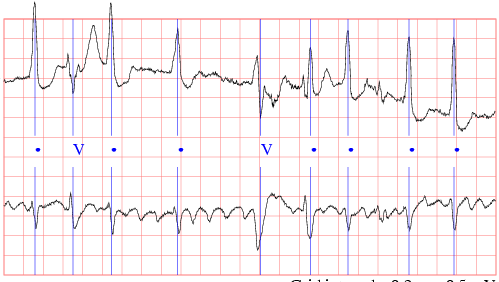
\includegraphics[width=0.9\linewidth]{mitdb.jpg}
	\caption{Fragment oznaczonych danych EKG z bazy MIT-BIH}
	\label{fig:mitdb}
\end{figure}

Do implementacji modelu analizy wykresów i sieci neuronowych wybrany został zestaw technologi Keras + Tensorflow. Umożliwia on bardzo łatwe tworzenie sieci neuronowych, co jeszcze bardziej zmniejsza czas potrzebny na przetestowanie różnych architektur sieci. Są to aktywnie rozwijane technologie posiadające bardzo rozległe możliwości, a przy tym posiadają szczegółowe dokumentacje. Dodatkowo biblioteki te są szeroko wykorzystywane w profesjonalnych rozwiązaniach co prowadzi do dużej liczby dostępnych informacji i aktywnego wsparcia.

\begin{figure}[h!]
	\centering
	
\includegraphics[width=0.8\linewidth]{keras-tensor.jpg}
	\caption{Technologie uczenia maszynowego}
	\label{fig:kt}
\end{figure}

Jako technologię do implementacji aplikacji i interfejsu użytkownika wybrana została biblioteka PySide2, dostarczająca interfejs dla języka Python do biblioteki Qt. Dzięki temu dostępna jest rozległa dokumentacja, której brakuje w innych rozważanych bibliotekach dla języka Python. Dodatkowo jest to biblioteka aktywnie rozwijana w przeciwieństwie do przestarzałej biblioteki dostępnej domyślnie w języku Python - Tkinter. Inną rozważaną opcją była biblioteka PyQt, jednak nie została ona finalnie wybrana, gdyż posiada zbyt restrykcyjną licencję GPL.

\begin{figure}[h!]
	\centering
	
\includegraphics[width=0.6\linewidth]{pyside.jpg}
	\caption{Biblioteka do interfejsu graficznego}
	\label{fig:pyside}
\end{figure}

Podsumowując, projekt niesie ze sobą dużą ilość wyzwań i niewiadomych. Z tego względu wybrany został model iteracyjny i szereg elastycznych technologii wspierających takie podejście. Wszystkie podjęte decyzje organizacyjne i technologiczne mają na celu zmniejszenie ryzyka i odpowiednie reagowanie na napotkane problemy. Umożliwia to określenie, że projekt jako całość z dużym prawdopodobieństwem zostanie wykonany, a wszelkie poważniejsze zagrożenia ograniczone będą do poszczególnych funkcjonalności i modułów.

\subsection{Analiza zagrożeń}

Podczas tworzenia aplikacji do predykcji arytmii w tak małym zespole istnieje wiele zagrożeń. Najistotniejsze z nich to:

\begin{itemize}
\item Brak wiedzy dziedzinowej - jako studenci informatyki nie posiadamy żadnej wiedzy z zakresu medycyny i chorób serca, nie wiemy szczegółowo jak działa ludzki organizm oraz jak pracuje narząd, który pompuje krew w jego wnętrzu. Może to bardzo utrudnić pracę oraz prowadzić do pewnych błędów w rozumowaniu.

\item Brak wystarczającej ilości danych - potrzebujemy dużej ilości danych, aby program mógł się nauczyć przewidywać arytmie. Dodatkowo dane te muszą być dokładnie oznaczone, gdyż nie jesteśmy w stanie zrobić tego sami, a bardzo ciężko o takie dane.

\item Niewystarczająca skuteczność sieci neuronowej - może się okazać że nie jesteśmy w stanie uzyskać skuteczności, która byłaby satysfakcjonująca, być może nie ma specjalnych prawidłowości, które pozwoliłyby przewidywać nieprawidłowości w pracy serca lub sieć neuronowa nie poradzi sobie z tak skomplikowanym problemem.

\item Różnorodność typów arytmii - rodzajów arytmii jest wiele, nie wszystkie są dokładnie zbadane i opisane. Prawdopodobnie niektórych nie da się przewidzieć i nie będziemy mogli brać wszystkich pod uwagę.
\end{itemize}
%\emph{Charakterystyka problemu, motywacja projektu (w tym przegląd
%istniejących rozwiązań prowadząca do uzasadnienia celu prac),
% wizja produktu, studium wykonalności i analiza zagrożeń.}

\section{\SectionTitleScope}
\label{sec:zakres-funkcjonalnosci}
\subsection{Charakterystyka użytkowników systemu}

W naszym systemie wyróżnia się tylko jednego głównego użytkownika. Korzysta on z programu na platformę Windows i ma dostęp do wszystkich funkcjonalności dostarczanych przez produkt.

\subsection{Wymagania funkcjonalne}

Wymagania funkcjonalne zostały przedstawione za pomocą historyjek użytkownika (ang. user stories), które określają co użytkownik chcę zrobić za pomocą systemu i w jakim celu.

\begin{itemize}
	\item Chcę wyświetlić zapisany wykres EKG żeby go przeanalizować
	\item Chcę zobaczyć wykres EKG aktualizowany w czasie rzeczywistym żeby na bieżąco widzieć jego zmiany i wyniki analizy
	\item Chcę zobaczyć oznaczenia poszczególnych uderzeń serca żeby lepiej zorientować się w wykresie i łatwiej odnaleźć interesujące fragmenty
	\item Chcę zobaczyć oznaczenia wykrytej arytmii serca żeby zlokalizować poszczególne epizody oraz móc łatwiej je przeanalizować
	\item Chcę zobaczyć podstawowe informację o poszczególnych arytmiach żeby lepiej zrozumieć wyniki analizy i odpowiednio na nie zareagować
	\item Chcę zobaczyć wyniki predykcji arytmii w przyszłości żeby odpowiednio wcześniej zareagować na spodziewane nieprawidłowości
\end{itemize}

\subsection{Wymagania niefunkcjonalne}

Wymagania aplikacji:

\begin{itemize}
	\item Musi działać na systemach Windows
	\item Interfejs musi być intuicyjny, przejrzysty i dostarczać wszystkich wymaganych informacji
	\item Wyświetlane wykresy muszą być skalowalne
\end{itemize}

Wymagania technologiczne:

\begin{itemize}
	\item Musi istnieć prosty sposób rozszerzania systemu o nowe formaty zapisu wykresów EKG
	\item System musi umożliwiać proste rozszerzanie o nowe metody analizy, w tym o różne algorytmy wykrywania i predykcji
\end{itemize}

\section{\SectionTitleRealizationAspects}
\label{sec:wybrane-aspekty-realizacji}
%\emph{Przyjęte założenia, struktura i zasada działania systemu,
%  wykorzystane rozwiązania technologiczne wraz z uzasadnieniem
%  ich wyboru, istotne mechanizmy i zastosowane algorytmy.} 
Projekt został podzielony na 3 główne moduły : 

\begin{itemize}
	\item interface - jest w pełni odpowiedzialny za interfejs graficzny
	\item model - zawiera wszystkie elementy dotyczące przetwarzania danych oraz predykcji
	\item experimental - znajduje się w nim kod odpowiedzialny za testowanie i trenowanie różnych konfiguracji sieci neuronowych
\end{itemize}

W odrębnym module znajdują się wszystkie napisane przez nas testy.

\subsection{Interfejs}

Interfejs graficzny składa się na 4 główne widoki: główne menu, okno predykcji, okno do przeglądania wykresów EKG oraz okno z mikro-biblioteką zawierającą informacje o uwzględnionych typach arytmii. Każdym widokiem zajmuje się osobna klasa, a wszystkimi widokami zarządza manager. Poza głównymi widokami w oknie predykcji dostępne są 2 dodatkowe widoki: okno z logami predykcji oraz okno wyboru modelu predykcji. Widoki zostały częściowo stworzone przy pomocy programu Qt Designer i zapisane w plikach formatu .ui. Są one ładowane z tych plików, a następnie odpowiednio modyfikowane już w kodzie.

\begin{figure}[H]
	\centering
	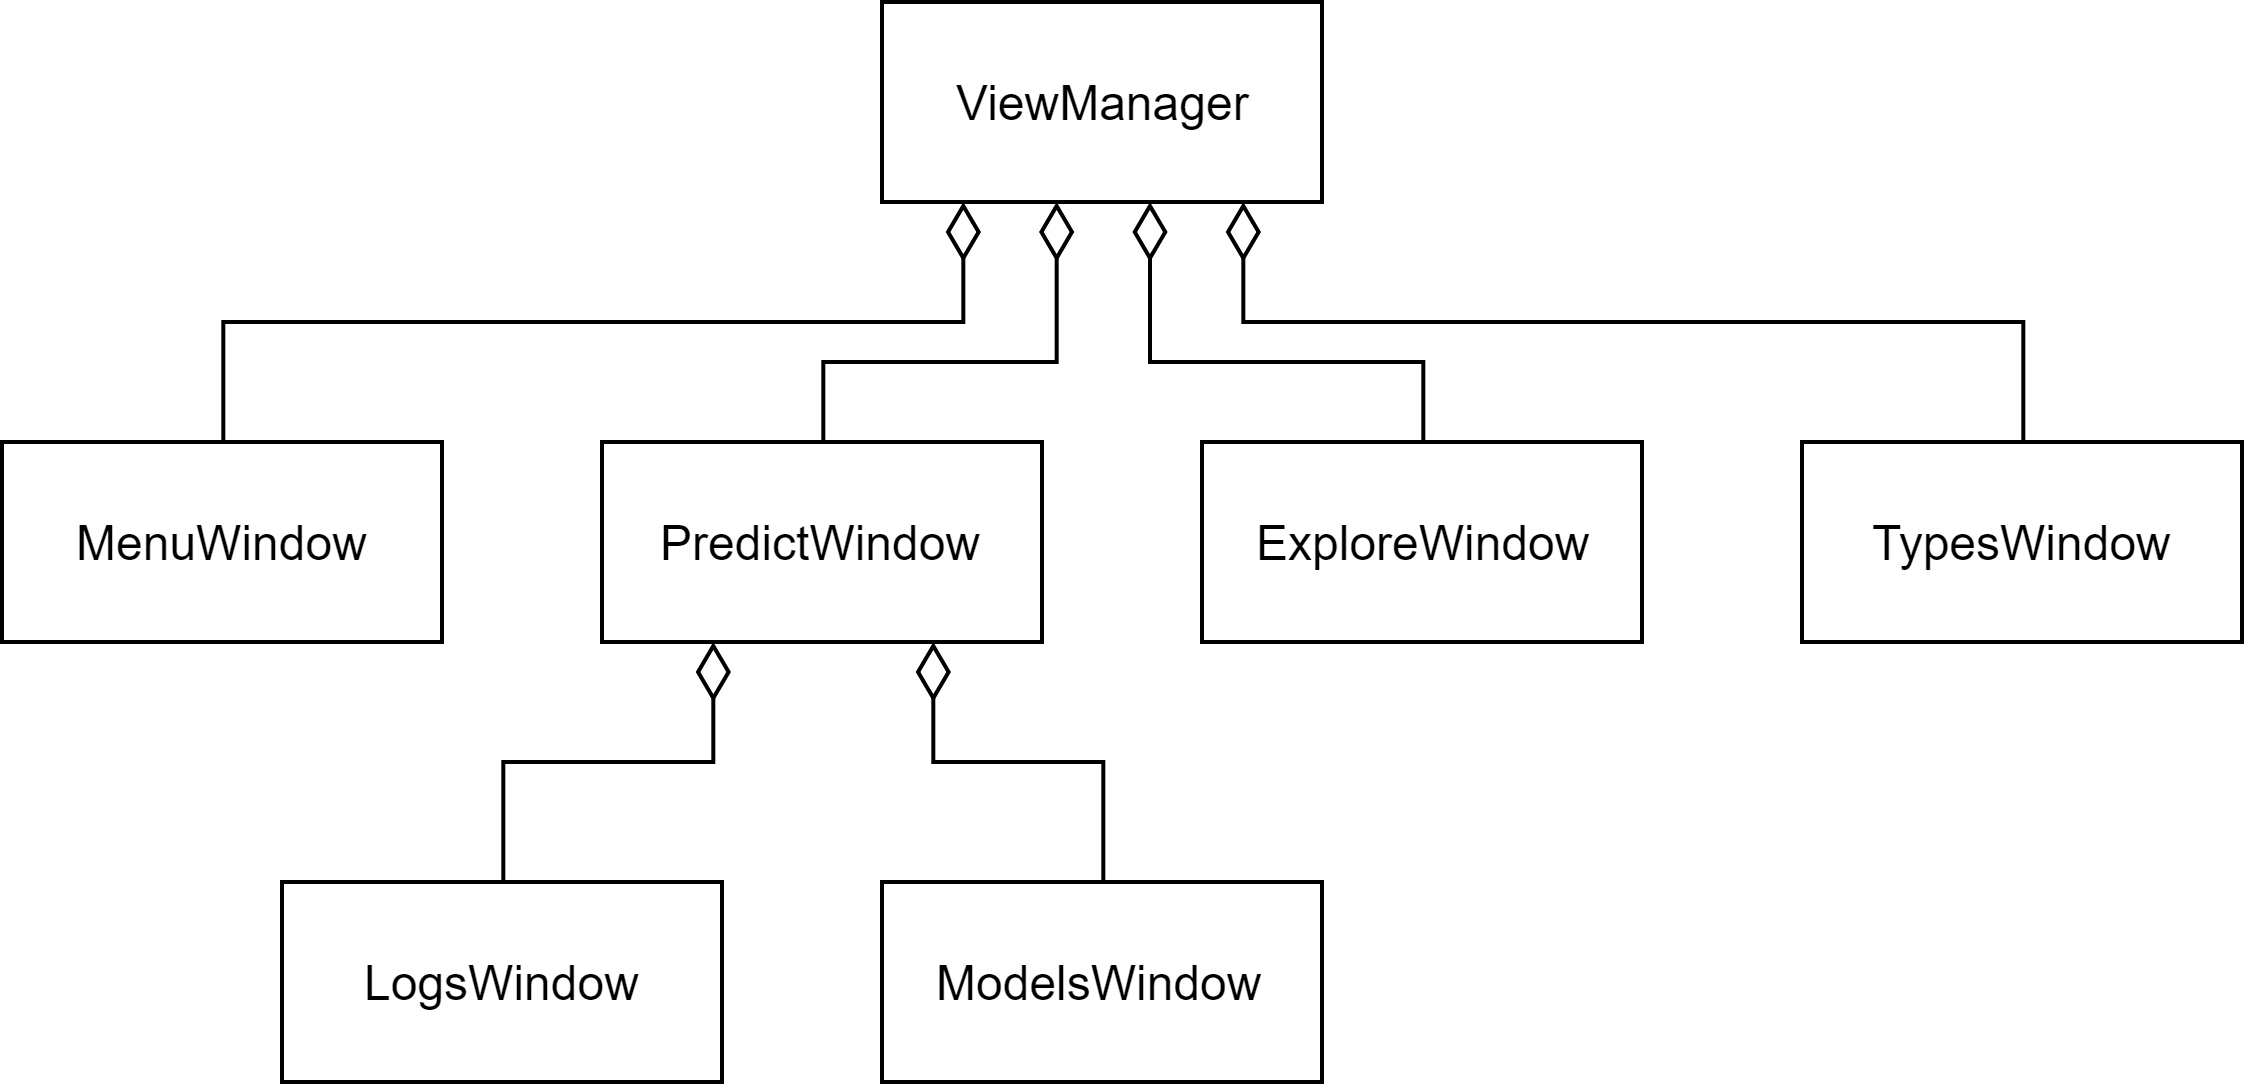
\includegraphics[width=0.8\linewidth]{interface_class_diagram.png}
	\caption{Diagram klas modułu interface}
	\label{fig:interface_diagram_class}
\end{figure}

\begin{lstlisting}[float=h!, caption={Kod managera widoków}]
class ViewManager(QStackedWidget):

    def __init__(self, *args, **kwargs):
        super().__init__(*args, **kwargs)
        self.menu = MenuWindow(self, load_ui('resources/menu.ui'))
        self.predict = PredictWindow(self, load_ui('resources/predict.ui'), load_ui('resources/logs.ui'), load_ui('resources/models.ui'))
        self.types = TypesWindow(self, load_ui('resources/types.ui'))
        self.explore = ExploreWindow(self, load_ui('resources/explore.ui'))

        self.addWidget(self.menu.window)
        self.addWidget(self.predict.window)
        self.addWidget(self.types.window)
        self.addWidget(self.explore.window)

        self.resize(1100, 700)
        self.setWindowTitle("Arrhythmia prediction")
        self.show()

    def show_menu(self):
        self.setCurrentWidget(self.menu.window)

    def show_predict(self):
        self.setCurrentWidget(self.predict.window)

    def show_types(self):
        self.setCurrentWidget(self.types.window)

    def show_explore(self):
        self.setCurrentWidget(self.explore.window)

    def closeEvent(self, event):
        self.explore.closeEvent()
        self.predict.closeEvent()
        
\end{lstlisting}

\begin{figure}[h!]
	\centering
	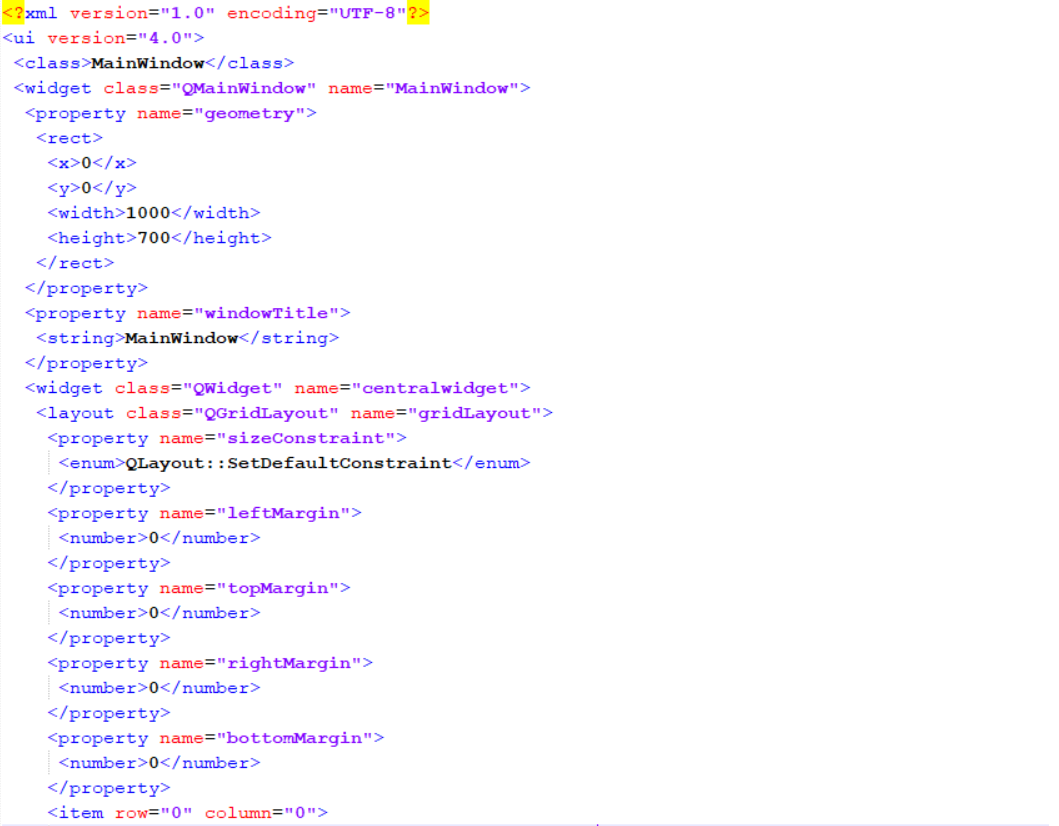
\includegraphics[width=0.9\linewidth]{ui_file.png}
	\caption{Przykładowy fragment pliku .ui}
	\label{fig:ui_file}
\end{figure}

\subsubsection{Główne menu}

Menu zawiera 4 przyciski i pozwala przełączać się pomiędzy głównymi widokami. Każdy z tych widoków umożliwia powrót do głównego menu.

\begin{figure}[h!]
	\centering
	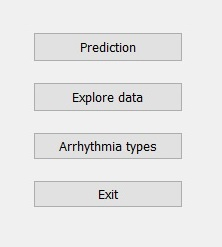
\includegraphics[width=0.3\linewidth]{menu.png}
	\caption{Główne menu programu}
	\label{fig:menu}
\end{figure}

\subsubsection{Okno predykcji}

Podstawowe i najważniejsze okno w programie. Umożliwia ono wczytanie danych EKG z pliku w formacie .dat(domyślny format bazy MIT-BIH z której korzystamy) poprzez wybranie go w eksploratorze plików.
 
Na podstawie wczytanych danych generowany jest wykres podglądu przedstawiający 6 sekundowy fragment rekordu. Wykres jest skalowany na osi Y do aktualnie wyświetlanych danych, tak aby były one zawsze dobrze widoczne. W prawym dolnym rogu tego wykresu znajduje się mniejszy wykres, wraz z legendą, przedstawiający jak zmieniały się poszczególne wartości predykcji na przestrzeni ostatnich 10 wartości. 

\begin{figure}[h!]
	\centering
	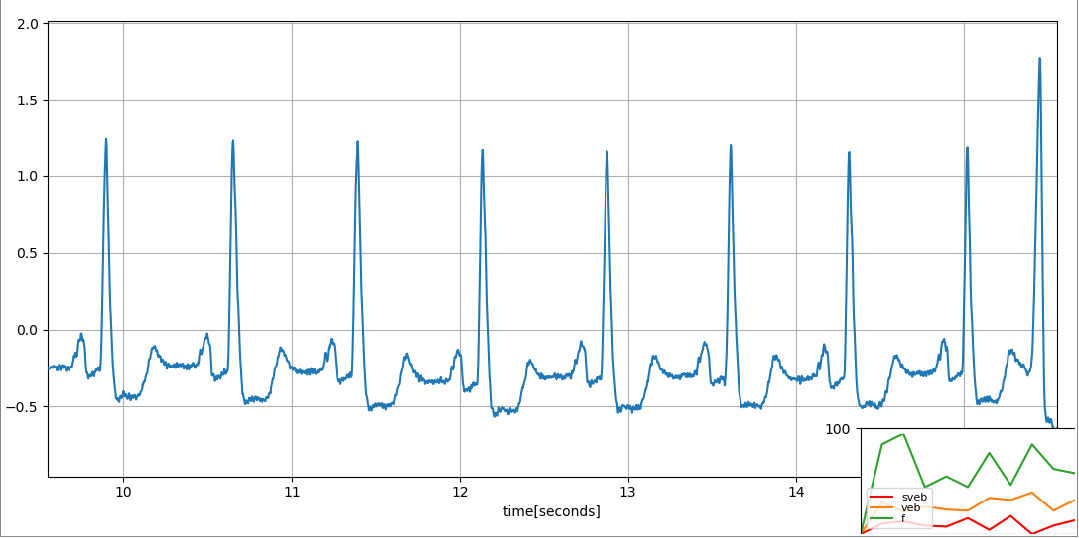
\includegraphics[width=0.9\linewidth]{plot.png}
	\caption{Wykres danych EKG wraz z wykresem zmian predykcji}
	\label{fig:plot}
\end{figure}

Nad wykresem znajduje się pasek nawigacyjny umożliwiający:
\begin{itemize}
\item przeskok do wybranego fragmentu poprzez wpisanie wartości początkowej wykresu w sekundach z dokładnością do 2 cyfr dziesiętnych, wartość jest ograniczona do rozmiaru danych
\item przewijanie wykresu wstecz lub do przodu poprzez klikanie bądź przytrzymanie odpowiedniego przycisku
\item odtwarzanie danych w przód co pozwala symulować działanie w czasie rzeczywistym
\end{itemize}

Dodatkowo po wczytaniu danych wyświetlana jest nazwa rekordu oraz maksymalna wartość do której można przeskoczyć. Odtwarzanie danych inicjowane jest przez odrębny wątek.

\begin{figure}[h!]
	\centering
	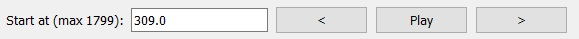
\includegraphics[width=0.9\linewidth]{navigation.png}
	\caption{Pasek do nawigacji po wykresie}
	\label{fig:navigation}
\end{figure}

Pod wykresem z prawej strony znajduje się pasek wyświetlający wartości, które na wyjściu daje model predykcji dla aktualnych danych. Rozważamy 3 typy arytmii o oznaczeniach: SVEB, VEB oraz F.
Predykcja również inicjowana jest w innym wątku i odbywa się co 1 sekundę w trakcie odtwarzania wykresu.

\begin{figure}[H]
	\centering
	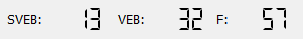
\includegraphics[width=0.5\linewidth]{output.png}
	\caption{Pasek wartości predykcji}
	\label{fig:output}
\end{figure}

Dodatkowo na dole znajduje się przycisk, który umożliwia otworzenie okna zawierające logi wszystkiego co się do tej pory działo w zakładce dotyczącej predykcji. W oknie mamy możliwość wyczyszczenia dotychczasowej historii lub zapisania jej do pliku tekstowego.

\begin{figure}[H]
	\centering
	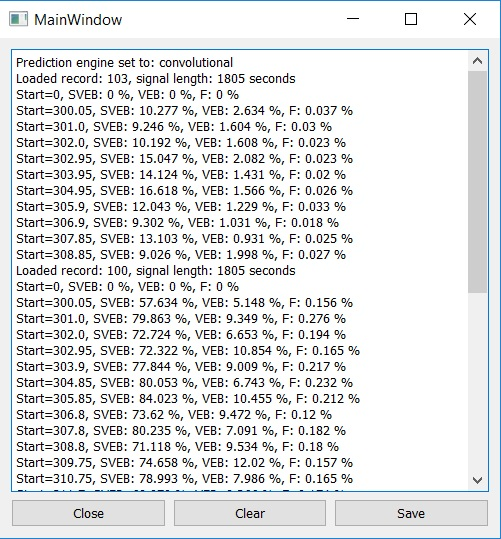
\includegraphics[width=0.6\linewidth]{logs.png}
	\caption{Okno wyświetlające logi programu}
	\label{fig:logs}
\end{figure}

\begin{figure}[H]
	\centering
	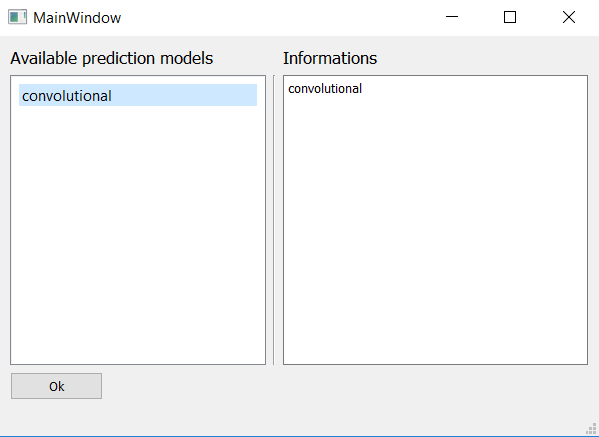
\includegraphics[width=0.6\linewidth]{models.png}
	\caption{Okno wyboru modelu predykcji}
	\label{fig:models}
\end{figure}

Całość prezentuje się następująco:

\begin{figure}[H]
	\centering
	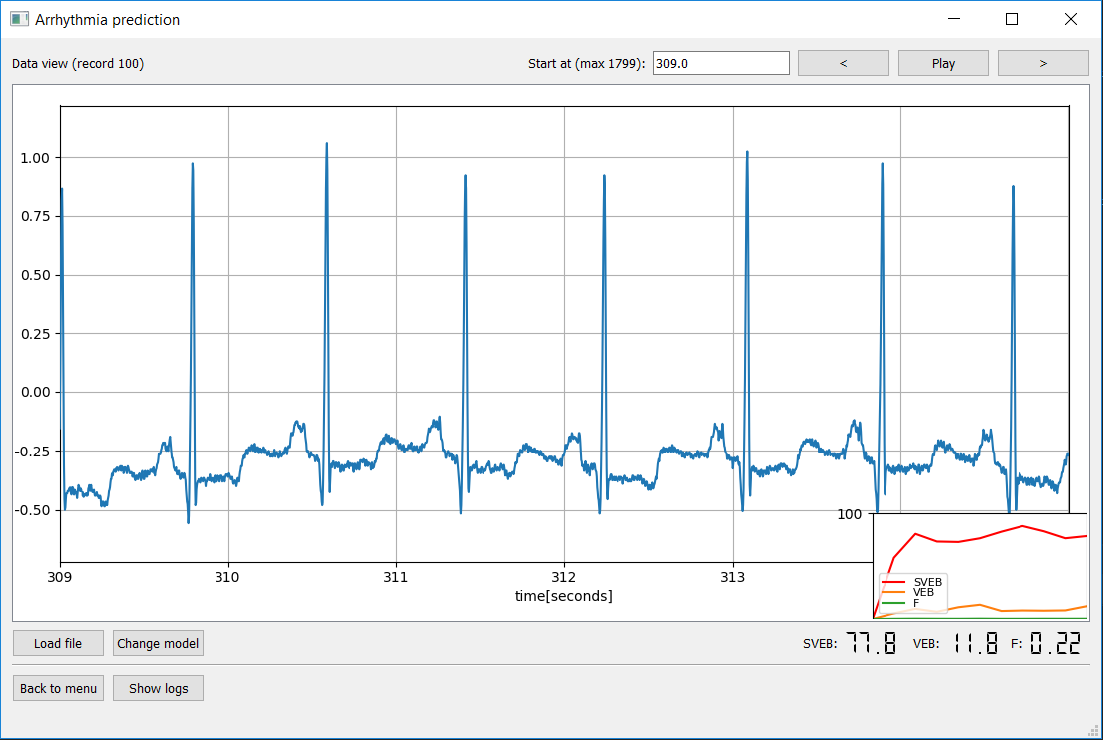
\includegraphics[width=0.9\linewidth]{prediction.png}
	\caption{Widok okna predykcji}
	\label{fig:prediction}
\end{figure}

\subsubsection{Przeglądanie danych}

W oknie tym mamy możliwość przeglądania bardziej szczegółowych danych. Umożliwia wczytanie danych z plików wraz z informacjami na temat poszczególnych uderzeń. Na podstawie danych generowany jest wykres na którym każde uderzenie jest oznaczone w odpowiedni sposób. Nad wykresem znajduje się pasek do nawigacji po wykresie taki sam jak w oknie predykcji.

\begin{figure}[h!]
	\centering
	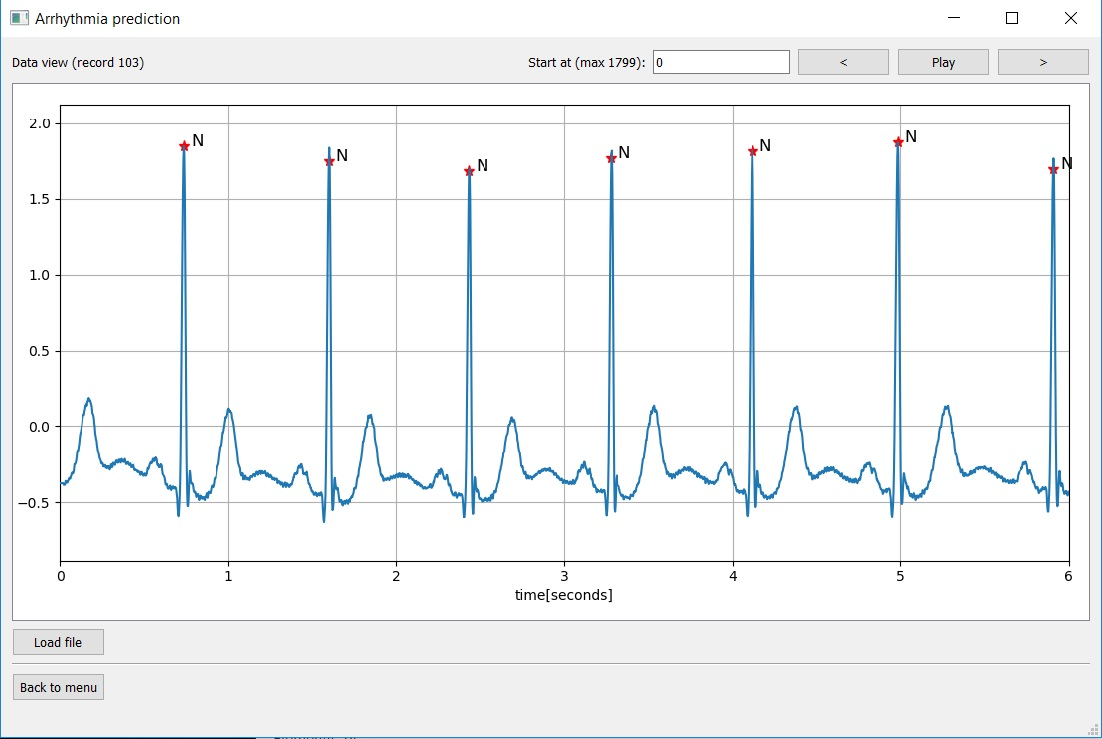
\includegraphics[width=0.8\linewidth]{explore.png}
	\caption{Okno do przeglądania oznaczonych danych}
	\label{fig:explore}
\end{figure}

\subsubsection{Dodatkowe informacje}

Jest to dodatkowe okno, będące małą biblioteką rozważanych przez nas typów arytmii. Z lewej strony mamy listę zawierającą rodzaje nieprawidłowości. Po wybraniu elementu z listy po prawej stronie zostaną wyświetlone odpowiednie informacje. Dane wczytywane są z plików tekstowych.

\begin{figure}[H]
	\centering
	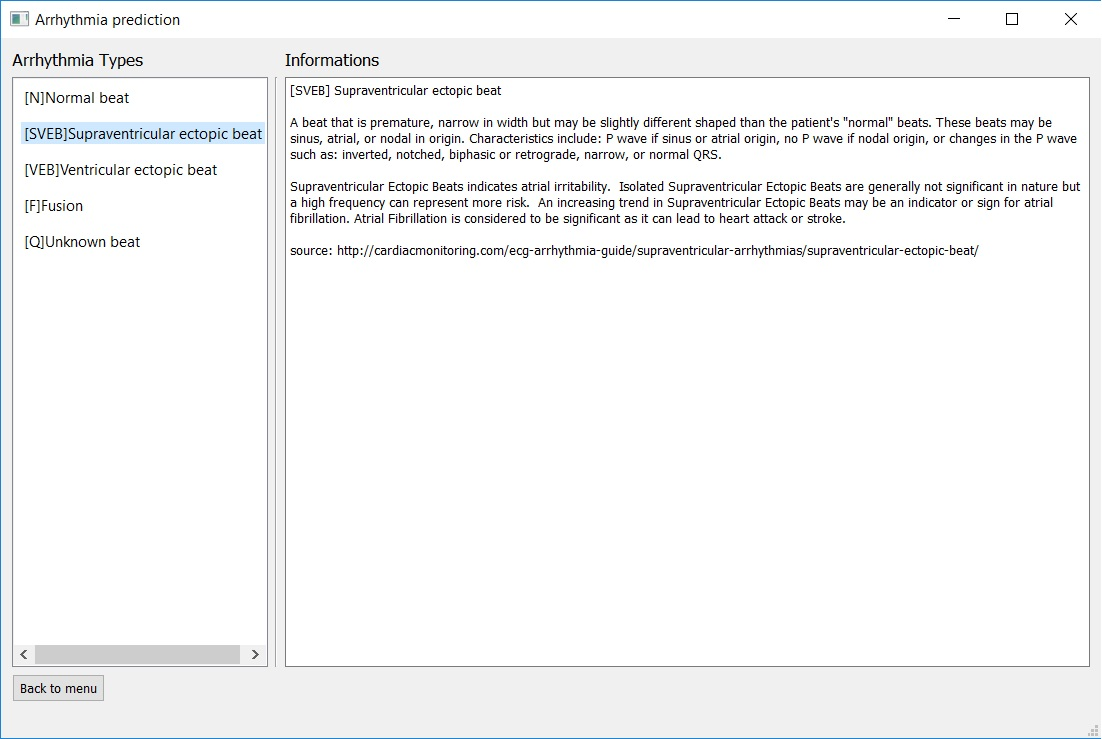
\includegraphics[width=0.7\linewidth]{types.png}
	\caption{Okno z informacjami na temat różnych typów arytmii}
	\label{fig:types}
\end{figure}

\subsection{Model}

Głównym zadaniem modułu modelu w systemie jest dostarczenie funkcjonalności umożliwiającej dokonywanie predykcji na podstawie wykresu EKG. W tym celu zdefiniowane zostało pojęcie silnika predykcji jako elementu dostarczającego taką funkcjonalność. Musi on dokonywać przetwarzania danych wejściowych, takiego jak likwidacja szumów i normalizacja, oraz wykonywać predykcji. Predykcją zwróconą przez silnik będzie ciąg wartości z przedziału od zera do jeden, o liczebności takiej samej jak ilość przewidywanych rodzajów arytmii. Każda wartość określać będzie szansę na wystąpienie danego rodzaju arytmii.

% FIXME Nie lubię tego "jak zostało wspomniane" vv
Ponieważ jak wynikło z analizy wykonalności projekt wymaga przetestowania dużej ilości sposobów dokonywania klasyfikacji, moduł modelu musi dostarczać możliwość stworzenia różnych silników predykcji. W tym celu konieczna jest funkcjonalność do łatwego tworzenia nowych silników. Dodatkowo model musi udostępniać reszcie systemu możliwość wyboru spośród dostępnych silników za pomocą jednolitego interfejsu.

\subsubsection{Zasada działania}

W celu zrealizowania założonych wymagań podjęta została decyzja o warstwowej budowie silnika predykcji. Przy takim założeniu moduł modelu dostarcza gotowych warstw, z których zbudowane mogą zostać różnego rodzaju silniki.  Na rysunku \ref{fig:model_example_flow}. przedstawiony został przykładowy schemat silnika predykcji ilustrujący przepływ danych. Znajdujące się na nim warstwy podane jako przykład to:

\begin{description}
	\item[Fragmentacja danych] - z wejściowych danych zostaje wydzielony fragment używany do predykcji. Rozmiar tego fragmentu odpowiada oknu na podstawie, którego wykonywana jest predykcja.
	\item[Zmniejszenie rozdzielczości] - częstotliwość próbek zmniejszona jest w celu redukcji ilości cech i likwidacji szumów wysokich częstotliwości. Przykładowo częstotliwość może zostać zmniejszona z \SI{360}{\hertz} do \SI{60}{\hertz} przez usunięcie wszystkich poza  co szóstą wartością.
	\item[Usuwanie niskich częstotliwości] - za pomocą transformaty Fouriera i jej odwrócenia likwidowane są niskie częstotliwości spowodowane między innymi przez oddech pacjenta. Przykładowo zlikwidowane mogą zostać częstotliwości poniżej \SI{0.3}{\hertz} poprzez wyzerowanie odpowiednich wartości po zastosowaniu szybkiej transformaty Fouriera.
	\item [Normalizacja danych] - przed wprowadzeniem danych do sieci neuronowej dane muszą zostać znormalizowane zgodnie z oczekiwaną normalizacją dla sieci. Przykładowa funkcja normalizująca to $f(x) = \frac{x - \overline{x}}{x_{\sigma}}$, gdzie $\overline{x}$ to średnia wartości $x$, a $x_{\sigma}$ to ich odchylenie standardowe.
	\item [Klasyfikacja] - sieć neuronowa dokonuje klasyfikacji wieloklasowej i jako rezultat otrzymywane są przewidywane szansę na wystąpienie danej arytmii w przewidywanym oknie, określonym w trakcie trenowania sieci.
\end{description}

\begin{figure}[h!]
	\centering
	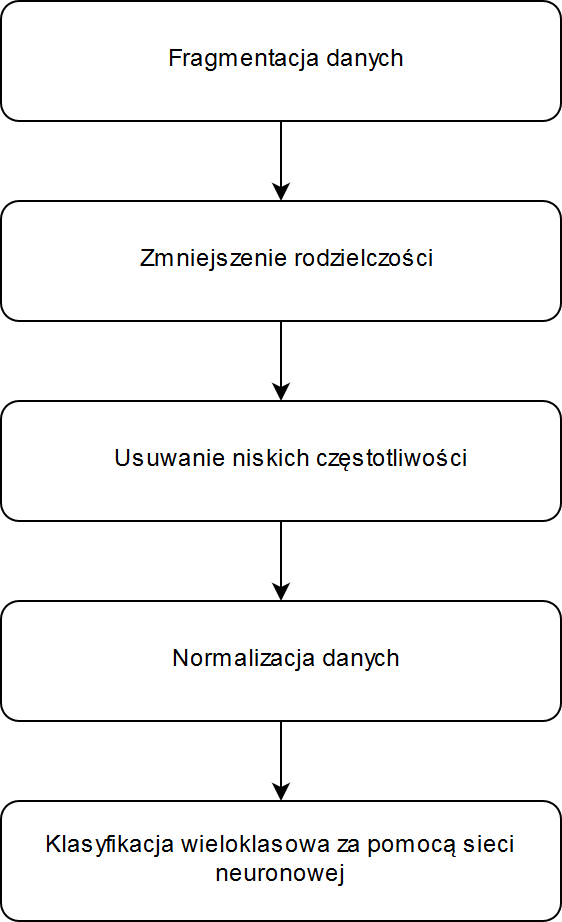
\includegraphics[width=0.4\linewidth]{model_example_flow.png}
	\caption{Schemat warstw w przykładowym silniku predykcji}
	\label{fig:model_example_flow}
\end{figure}

W celu umożliwienia takiej modułowości dla budowy silników predykcji zdefiniowany został wspólny interfejs dla wszystkich warstw i zrealizowany jako abstrakcyjna klasa \emph{Layer}. Jej podstawowym założeniem jest przetwarzanie danych i przekazywanie ich do następnych warstw w ciągu. W tym celu posiada ona następujące metody:

\begin{itemize}
	\itemsep0em
	\item[] \emph{set\_next(Layer)} - ustawia następny obiekt w silniku, do którego przekazywane będą wyniki obliczeń
	\item[] \emph{push\_value(Numpy array)} - dostarcza obiekt na którym wykonane zostaną obliczenia, a ich wynik zostanie przekazany dalej
	\item[] \emph{compute(Numpy array): Numpy array} - abstrakcyjna metoda, która w klasach dziedziczących powinna wykonywać zadane obliczenie i zwracać wynik
\end{itemize}

W trakcie tworzenia nowych silników predykcji stworzone zostały odpowiednie warstwy wewnątrz modelu, umożliwiając ich ponowne wykorzystanie. Rysunek \ref{fig:pipes_uml} zawiera diagram klas przedstawiający relację między klasami implementującymi  warstwy wewnątrz modelu, zaś poniżej znajdują się ich szczegółowe opisy.

\begin{figure}[h!]
	\centering
	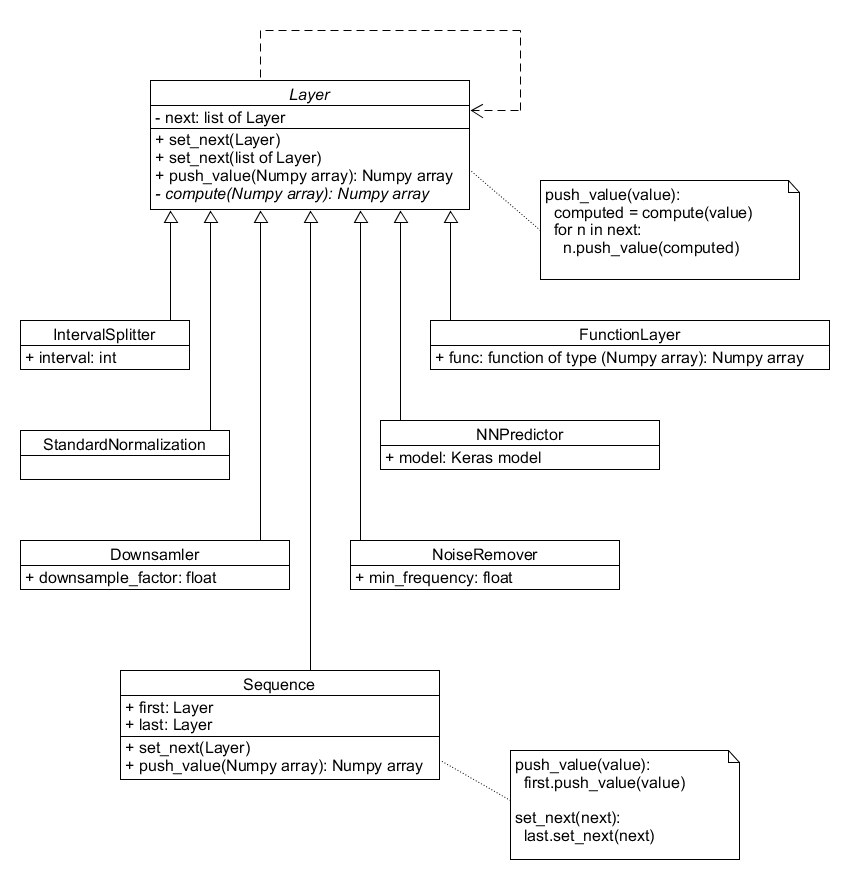
\includegraphics[width=0.8\linewidth]{pipes_uml.png}
	\caption{Diagram klas dla warstw modelu}
	\label{fig:pipes_uml}
\end{figure}

\paragraph{IntervalSplitter} Początkowa warstwa, dokonująca wycięcia z wejściowych danych okna zadanego rozmiaru. Na wejściu otrzymuje ona cały dotychczasowy wykres EKG, z którego przekazywany dalej zostaje tylko ostatni fragment o rozmiarze oczekiwanym przez następne warstwy i klasyfikator.

\paragraph{StandardNormalizer} Jest to warstwa dokonująca normalizacji danych za pomocą tzw. \emph{standaryzacji Z}. Wzór określający ten rodzaj normalizacji to $f(x) = \frac{x - \overline{x}}{x_{\sigma}}$, gdzie $\overline{x}$ to wartość średnia, zaś $x_\sigma$ to odchylenie standardowe. Dzięki zastosowaniu takiej normalizacji wyjściowe wartości posiadają średnią równą zero, zaś odchylenie standardowe równe jeden. Ten rodzaj normalizacji jest szczególnie przydatny przy przetwarzaniu danych dla sieci neuronowych z warstwami zawierającymi jako aktywacje funkcję \emph{ReLU - Rectified Linear Unit}.

% TODO Wstawić rysunek prezentujący działanie i może kod

\paragraph{Downsampler} Warstwa odpowiadająca za redukcję częstotliwości. Dzięki jej zastosowaniu jesteśmy w stanie znacząco przyśpieszyć działanie sieci neuronowej oraz zmniejszyć wymiarowość danych. Oba te efekty pomagają zredukować wpływ \emph{przekleństwa wymiaru} spowodowanego ogromną ilością cech w wejściowym fragmencie EKG. Dodatkowo zmniejszenie ilości próbek pozwala usunąć szum w wysokich częstotliwościach spowodowany przez zakłócenia elektroniczne lub niedoskonałości w trakcie analogowego zapisu i późniejszej digitalizacji.
Rysunek \ref{fig:downsampling} prezentuje efekt redukcji częstotliwości na przykładzie pięciosekundowego wycinka wykresu.

% TODO Wykonać wykres z większą rozdzielczością, poprawić tytuł i oznaczenia osi x.
\begin{figure}[h!]
	\centering
	\captionsetup{justification=centering}
	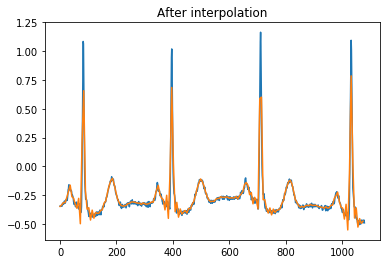
\includegraphics[width=0.6\linewidth]{downsampling.png}
	\caption{Redukcja częstotliwości z \SI{360}{\hertz} (niebieski wykres) do \SI{60}{\hertz} (pomarańczowy wykres)}
	\label{fig:downsampling}
\end{figure}

\paragraph{NoiseRemover} Jest to warstwa usuwająca szum niskich częstotliwości, który spowodowany jest oddechem pacjenta, zmianą położenia i czynnikami zewnętrznymi obecnymi w trakcie nagrywania zapisu. Operacja ta została zaimplementowana za pomocą transformaty Fouriera. W pierwszej kolejności wejściowy fragment przekształcany jest do domeny częstotliwości, następnie zerowane są wartości poniżej wybranej granicznej częstotliwości. Po usunięciu odpowiedniego przedziału wykonywana zostaje odwrotna transformata Fouriera, przywracająca fragment do domeny czasu. Na rysunku \ref{fig:fft} widoczne jest działanie tej warstwy na przykładzie fragmentu EKG, zaś rysunek \ref{fig:fft_f} przedstawia ten sam fragment przedstawiony w dziedzinie częstotliwości po zastosowaniu transformaty.

\begin{figure}[h!]
	\centering
	\captionsetup{justification=centering}
	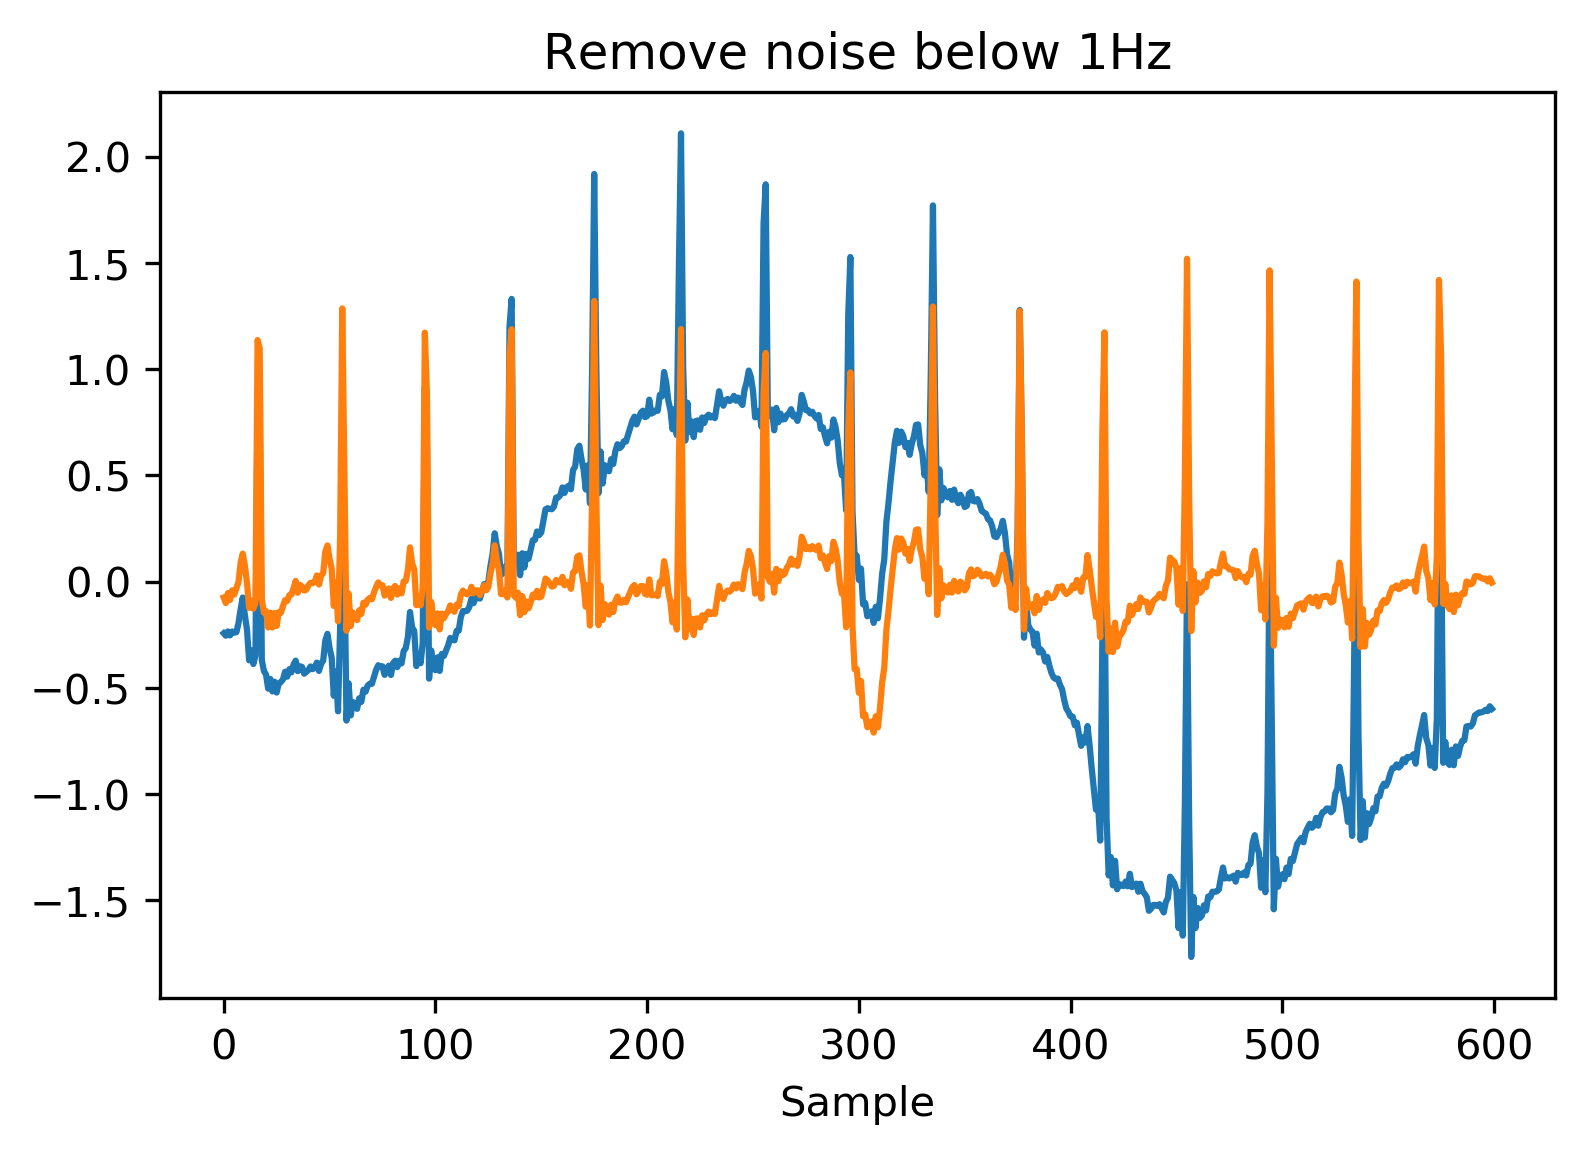
\includegraphics[width=0.6\linewidth]{noise_remove.png}
	\caption{Usunięcie częstotliwości poniżej \SI{0,5}{\hertz} za pomocą transformaty Fouriera. Kolor niebieski - oryginalny fragment, kolor pomarańczowy - po wycięciu niskich częstotliwości.}
	\label{fig:fft}
\end{figure}

\begin{figure}[h!]
	\centering
	\captionsetup{justification=centering}
	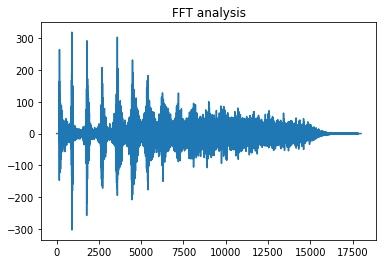
\includegraphics[width=0.6\linewidth]{fft_fdomain.png}
	\caption{Widok fragmentu wykresu EKG w dziedzinie częstotliwości}
	\label{fig:fft_f}
\end{figure}

\paragraph{NNPredictor} Warstwa zawierająca klasyfikator w postaci sieci neuronowej. Odpowiada ona za integrację z biblioteką Keras, w tym celu dokonuje zmiany kształtu danych wejściowych do tego oczekiwanego przez sieć. Wszystkie sieci używane w modelu są wcześniej wytrenowane w module eksperymentów, warstwa ta więc wczytuje budowę sieci oraz wagi z pliku w formacie \emph{HDF5}. % TODO Dodać odnośnik do opisu formatu %

\paragraph{FunctionLayer} Pomocnicza warstwa służąca jedynie do integracji z pozostałymi elementami systemu. Nie przekształca ona danych, a jej jedyną funkcjonalnością jest wywołanie zewnętrznej funkcji, przekazując jako argument rezultat poprzednich warstw.

\paragraph{Sequence} Pomocnicza warstwa tworząca abstrakcję nad grupą innych warstw. W jej wypadku wykonanie obliczeń jest równoznaczne wykonaniu obliczeń przez wszystkie warstwy które w sobie zawiera. Dzięki jej zastosowaniu interfejs dla sekwencji warstw jest taki sam jak dla pojedynczej warstwy. Jest to przydatne ponieważ silnik wewnątrz modelu zdefiniowany jest jako ciąg warstw, dzięki takiej abstrakcji silnik wykorzystuje istniejący interfejs, co zwiększa czytelność kodu i pomaga w integracji z resztą systemu.

Dla pozostałych modułów wyznaczony został interfejs służący do wyświetlenia dostępnych silników, stworzenia żądanego silnika oraz integracji jego funkcjonalności z obecną strukturą. Poniżej znajduje się szczegółowy opis elementów tego interfejsu, zaś na fragmencie 2. widoczny jest kod definiujący interfejs oraz przykładowy silnik predykcji.

\begin{itemize}
	\itemsep0em
	\item[] \emph{PredictionEngine} - klasa definiująca silnik predykcji, zawiera jego nazwę, opis i warstwy z których się składa
	\item[] \emph{engines} - lista dostępnych silników predykcji
	\item[] \emph{create\_prediction\_engine(PredictionEngine)} - pomocnicza funkcja budująca silnik, wczytuje klasyfikator oraz łączy ze sobą warstwy
	\item[] \emph{FunctionLayer} - klasa umożliwiająca dołączenie na końcu silnika wywołania funkcji z wynikiem predykcji
\end{itemize}

\begin{lstlisting}[float=h, style=custompy, caption=Interfejsu modelu i przykład wykorzystania]
# Przykład definicji silnika:
engines = [
    PredictionEngine('convolutional', [
        IntervalSplitter(360*60*5, 360),
        Downsampler(360, 60),
        NoiseRemover(60, 0.5),
        StandardNormalizer(),
        networks[0].load()]),
    # ...
]


def create_prediction_engine(engine):
    return engine.build()

# Stworzenie silnika predykcji:
p_engine = create_prediction_engine(engines[0])

# Przykład integracji - tutaj wypisanie wyników
p_engine.set_next(FunctionLayer(print))

values = # Wartości fragmentu EKG

# Wywołanie obliczeń:
p_engine.push_value(values)
\end{lstlisting}

\subsubsection{Silniki predykcji}

Model udostępnia różne silniki predykcji różniące się strukturą, algorytmem, rozmiarami przedziałów danych i skutecznością. Silniki zostały podzielone na dwie grupy w zależności od budowy sieci neuronowej, którą wykorzystują. Są to silniki gęste i konwolucyjne. Poniżej znajdują się ogólne opisy każdej grupy, budowa udostępnianych silników, wykorzystywanych sieci oraz ich skuteczność. Opis metodologii testowania, dokładniejsze rezultaty testów oraz wszystkie wypróbowane architektury znajdują się w dziale \ref{sec:experimental} - Eksperymenty.

\paragraph{Gęste}

Jako pierwsze utworzone zostały silniki predykcji oparte na sieciach neuronowych zbudowanych z gęstych warstw (ang. \emph{dense}). W warstwach tych wszystkie wartości wyjściowe obliczane są na podstawie wszystkich danych wejściowych. Matematycznie warstwa gęsta zdefiniowana jest jako:
$$
out = f_a(A \cdot in + bias)
$$
, gdzie $f_a$ to funkcja aktywacji, $A, bias$ to wewnętrzne wartości warstwy aktualizowane w trakcie uczenia, $in, out$ to kolejno wejście i wyjście gęstej warstwy. 

W warstwie gęstej neurony \emph{łączą} każdą wartość wejściową z każdą wartością wyjściową, z tego powodu ilość parametrów w sieci zbudowanej z takich warstw rośnie bardzo szybko wraz ze wzrostem złożoności i wymiarowości danych. Z tego powodu sieć taka jest bardzo podatna na przetrenowania, to znaczy wyuczenie się zbioru treningowego zamiast zależności jakie reprezentuje. Dodatkowo sieć taka traktuje w ten sam sposób zależność między odległymi wartościami w danych wejściowych, a wartościami sąsiednimi. Z tego powodu sieć ta niezbyt dobrze nadaje się do klasyfikacji wykresów zależnych od czasu tak jak w naszym przypadku.

\begin{table}[h]
	\centering
\begin{tabular}{l|lllll}
	Nazwa & Wejście & Okres predykcji & Częstotliwość & Redukcja szumów & Skuteczność \\ \hline
	dense1 & 5 minut & 2 minuty & \SI{60}{\hertz} & < \SI{1}{\hertz} & \SI{69,00}{\percent} \\
	dense2 & 3 minuty & 1 minuta & \SI{60}{\hertz} & < \SI{1}{\hertz} & \SI{73,48}{\percent}
\end{tabular}
\caption{Silniki predykcji oparte o gęste sieci neuronowe}
\label{tab:dense_engines}
\end{table}

\begin{table}[h]
	\centering
\begin{tabular}{l|ll}
	Warstwa      & Parametry             & Aktywacja \\ \hline
	Dense        & units = 100           & relu         \\
	Dense        & units = 200           & relu         \\
	Dense        & units = 100           & relu         \\
	Dense        & units = 3             & sigmoid
\end{tabular}
\caption{Warstwy w sieci gęstej dla silników \emph{dense1} i \emph{dense2}}
\label{tab:dense1}
\end{table}

\paragraph{Konwolucyjne}

W konwolucyjnych silnikach predykcji głównym założeniem było wykorzystanie konwolucyjnej sieci neuronowej. Spowodowane było to bardzo słabymi wynikami dla gęstych sieci z powodu przetrenowania oraz sekwencyjną strukturą danych. Sieci konwolucyjne pozwalają bardzo dobrze klasyfikować dane, gdzie ważne jest wzajemne położenie cech, czyli w naszym przypadku odległość między wartościami na wykresie EKG. Innym przypadkiem przydatności takiej reprezentacji jest klasyfikacja obrazów, gdzie bardziej istotne są sąsiednie piksele niż te znajdujące się na osobnych końcach.

Głównymi częściami składowymi w konwolucyjnych sieciach neuronowych są warstwy wykonujące konwolucję oraz warstwy redukujące ich rozmiar przez tzw. \emph{pooling}. W kontekście przetwarzania danych EKG, wykonywaliśmy konwolucji w jednym wymiarze. Polega ona na sumie iloczynów wartości filtra i fragmentu wejściowych danych. Wyjściowa sekwencja jest ciągiem wyników takich operacji dla kolejnych fragmentów wejścia. Ilustracja działania konwolucji znajduje się na rysunku \ref{fig:convolution}.

\begin{figure}[h]
	\centering
	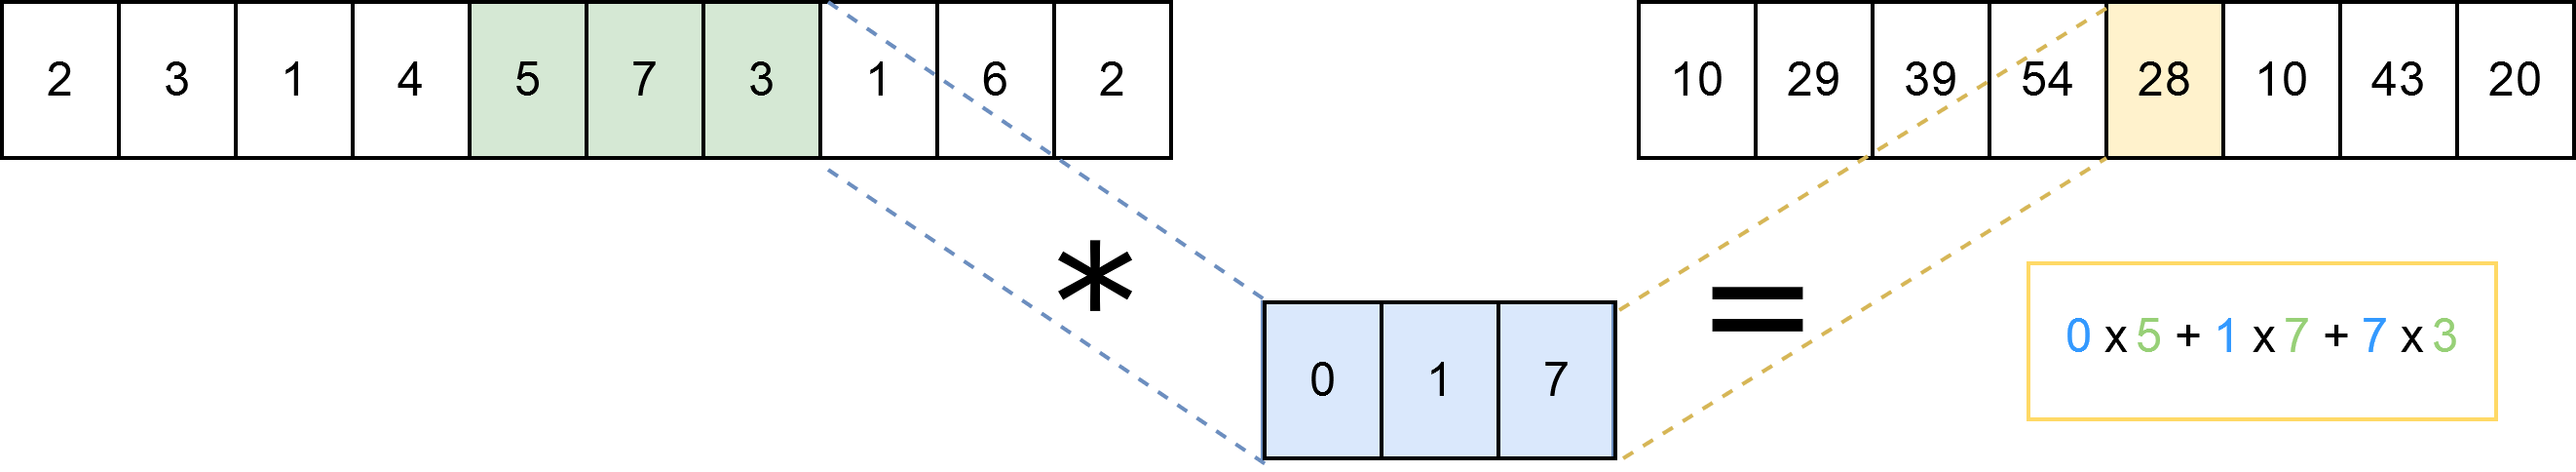
\includegraphics[width=\linewidth]{convolution.png}
	\caption{Działanie konwolucji w jednym wymiarze, dla rozmiaru filtra 3 i przesunięcia 1}
	\label{fig:convolution}
\end{figure}

Dodatkowo pojedyncza warstwa konwolucyjna może składać się z dowolnej ilości filtrów, wyjściem jest więc ciąg sekwencji. W celu zmniejszenia ilości wyjściowych danych jako następną warstwę stosuje się \emph{pooling}.
W naszym wypadku wykorzystaliśmy warstwy \emph{max-poolingu}, które wybierają największą wartość z zadanego przedziału i podobnie jak konwolucje produkują ciąg wartości dla przesuniętych przedziałów. Działanie tej operacji ilustruje rysunek \ref{fig:max_pool}.

\begin{figure}[h]
	\centering
	\captionsetup{justification=centering}
	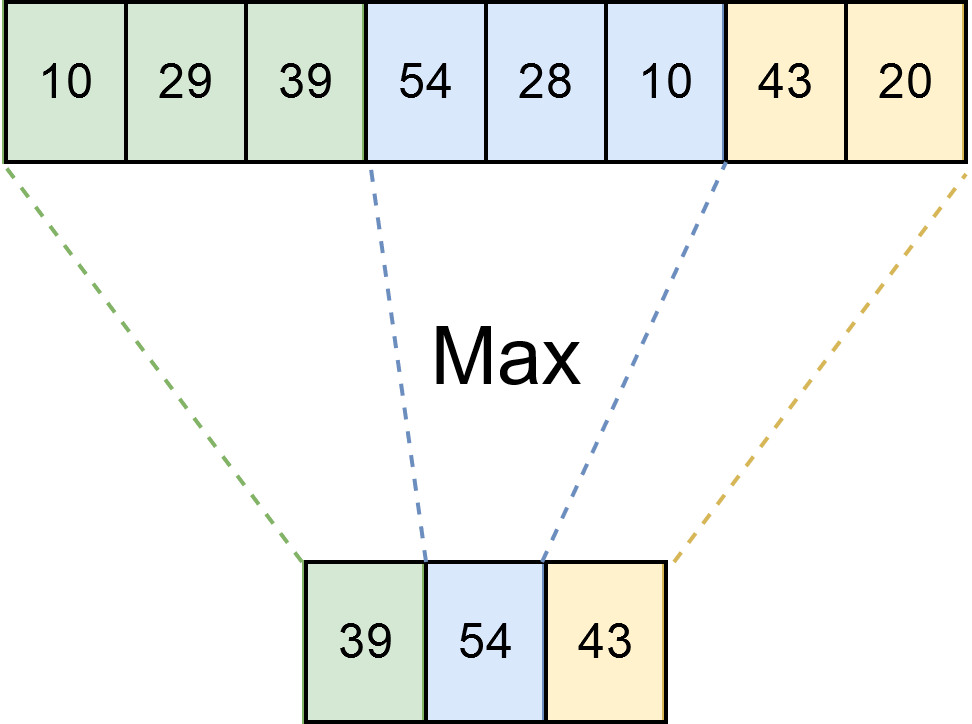
\includegraphics[width=0.4\linewidth]{max_pool.png}
	\caption{Działanie operacji 'max-pool' w jednym wymiarze, dla przedziału 3 i przesunięcia 3}
	\label{fig:max_pool}
\end{figure}

% TODO Opisać silniki dostępne w modelu

\begin{table}[h]
	\centering
\begin{tabular}{l|lllll}
	Nazwa & Wejście & Okres predykcji & Częstotliwość & Redukcja szumów & Skuteczność \\ \hline
	conv1 & 5 minut & 2 minuty & \SI{60}{\hertz} & < \SI{1}{\hertz} & \SI{84.21}{\percent} \\
	conv2 & 3 minuty & 1 minuta & \SI{60}{\hertz} & < \SI{1}{\hertz} & \SI{85.06}{\percent}
\end{tabular}
\caption{Silniki predykcji oparte o gęste sieci neuronowe}
\label{tab:conv_engines}
\end{table}

\begin{table}[h!]
	\centering
\begin{tabular}{l|ll}
	Warstwa      & Parametry                       & Aktywacja \\ \hline
	Reshape      & -                               & -         \\
	Conv1D       & kernels = 16, filter\_size = 16 & relu \\
	MaxPooling1D & pool\_size = 8                  & - \\
	Conv1D       & kernels = 8, filter\_size = 16  & relu \\
	MaxPooling1D & pool\_size = 8                  & - \\
	Conv1D       & kernels = 8, filter\_size = 16  & relu \\
	MaxPooling1D & pool\_size = 8                  & - \\
	Flatten      & -                               & - \\
	Dense        & units = 3                       & sigmoid
\end{tabular}
\caption{Warstwy w sieci konwolucyjnej dla silnika \emph{conv1}}
\label{tab:conv1}
\end{table}

\begin{table}[h!]
	\centering
\begin{tabular}{l|ll}
	Warstwa      & Parametry                       & Aktywacja \\ \hline
	Reshape      & -                               & -         \\
	Conv1D       & kernels = 32, filter\_size = 16 & relu \\
	MaxPooling1D & pool\_size = 16                 & - \\
	Conv1D       & kernels = 16, filter\_size = 16 & relu \\
	MaxPooling1D & pool\_size = 16                 & - \\
	Flatten      & -                               & - \\
	Dense        & units = 3                       & sigmoid
\end{tabular}
\caption{Warstwy w sieci konwolucyjnej dla silnika \emph{conv2}}
\label{tab:conv2}
\end{table}

\subsection{Eksperymenty} \label{sec:experimental}

\subsubsection{Baza treningowa}

Jako bazę treningową wykorzystaliśmy ogólnodostępną bazę danych EKG z oznaczonymi danymi - MIT-BIH Arrhythmia Database. Baza ta zawiera 48 pół-godzinnych, 2 kanałowych zapisów EKG. 23 rekordy zostały wybrane losowo ze zbioru 4000 24-godzinnych nagrań. Pozostałe 25 rekordów został wybranych z tego samego zbioru, jednak zawierających rzadsze, ale również klinicznie istotne przypadki arytmii.

Rekordy zostały zapisane z częstotliwością 360 próbek na sekundę, dla każdego z kanałów z 11 bitową rozdzielczością w zakresie 10mV. Każde nagranie zostało niezależnie oznaczone przez 2 lub więcej kardiologów. Sprzeczności zostały rozwiązane w taki sposób aby uzyskać czytelne komputerowo referencje dla każdego uderzenia znajdującego się w bazie. W przybliżeniu jest to 110,00 oznaczeń w całej bazie.
%TODO źródło: MIT-BIH

Dla każdego rekordu w bazie znajdują się 3 pliki:

\begin{itemize}
	\item plik .dat zawierający wartości kolejnych próbek
	\item plik .atr zawierający oznaczenie typu arytmii oraz miejsce jej wystąpienia na przebiegu EKG
	\item plik .hea zawierający nagłówek opisujący format danych
\end{itemize}

Do pobrania danych z sieci wykorzystaliśmy gotową bibliotekę wfdb napisaną w języku Python, która umożliwia w bardzo prosty sposób pobranie całej bazy.

\subsubsection{Typy arytmii}

Baza MIT-BIH zawiera dane z oznaczeniami 15 różnych typów uderzeń serca. Jest to zbyt duża ilość, aby uwzględniać je wszystkie. Postanowiliśmy więc zastosować standard AAMI i przekształcić dane w odpowiedni sposób.

Zawęziło to zbiór typów uderzeń do 5:

\begin{itemize}
	\item N - Normal beat
	\item SVEB- Supraventricular ectopic beat
	\item VEB - Ventricular ectopic beat
	\item F - Fusion
	\item Q - Unknown beat
\end{itemize}

\begin{lstlisting}[float=h!, caption={Kod mapujący oznaczenia z bazy MIT-BIH do standardu AAMI}]
mapping = {
	BeatType('N', 'Normal beat'): {'N', 'L', 'R'},
	BeatType('SVEB', 'Supraventricular ectopic beat'): {'e', 'j', 'A', 'a', 'J', 'S'},
	BeatType('VEB', 'Ventricular ectopic beat'): {'V', 'E'},
	BeatType('F', 'Fusion'): {'F'},
	BeatType('Q', 'Unknown beat'): {'/', 'f', 'Q'}
	}

def mit_to_aami(symbol):
	for key, value in mapping.items():
		if symbol in value:
			return key
	return None
	
\end{lstlisting}
 
\subsubsection{Podział danych}

Aby w pełni wykorzystać dane znajdujące się w bazie, każdy rekord jest dzielony na fragmenty o określonej długości, wybierane co określony krok czasowy. W ten sposób otrzymujemy wiele unikalnych fragmentów stanowiących podciągi całego rekordu.

\begin{lstlisting}[float=h!, caption={Funkcja dzieląca rekordy na fragmenty}]
def slice_records(records, pred_len, post_len, increment=360*60, check_pred=True):
    for record in records:
        for start in range(0, len(record[0]) - pred_len - post_len, increment):
            pred_end = start + pred_len
            post_end = pred_end + post_len
             pred = record[0][start:pred_end]
            post = record[0][pred_end:post_end]
             pred_inds = np.logical_and(start <= record[1], record[1] < pred_end)
            post_inds = np.logical_and(pred_end <= record[1], record[1] < post_end)
            if check_pred:
                pred_labels = record[2][pred_inds]
                if np.all(pred_labels == 'N'):
                    pred_result = pred, record[1][pred_inds], pred_labels
                    post_result = post, record[1][post_inds], record[2][post_inds]
                    yield pred_result, post_result
            else:
                pred_result = pred, record[1][pred_inds], record[2][pred_inds]
                post_result = post, record[1][post_inds], record[2][post_inds]
                yield pred_result, post_result

\end{lstlisting}

Dzieląc dane na treningowe i testowe zdecydowaliśmy się zastosować K-krotną walidacje krzyżową (z ang. K-fold cross-validation). Polega ona na tym że oryginalny zbiór jest dzielony na K podzbiorów. Następnie każdy z nich jest brany jako zbiór testowy, a pozostałe razem stanowią zbiór uczący. Odbywa się więc K iteracji, których wyniki są następnie uśredniane w celu uzyskania ostatecznego wyniku. W naszym wypadku jako parametr $K$ oraz ilość iteracji wybraliśmy wartość 5.

\begin{figure}[h!]
	\centering
	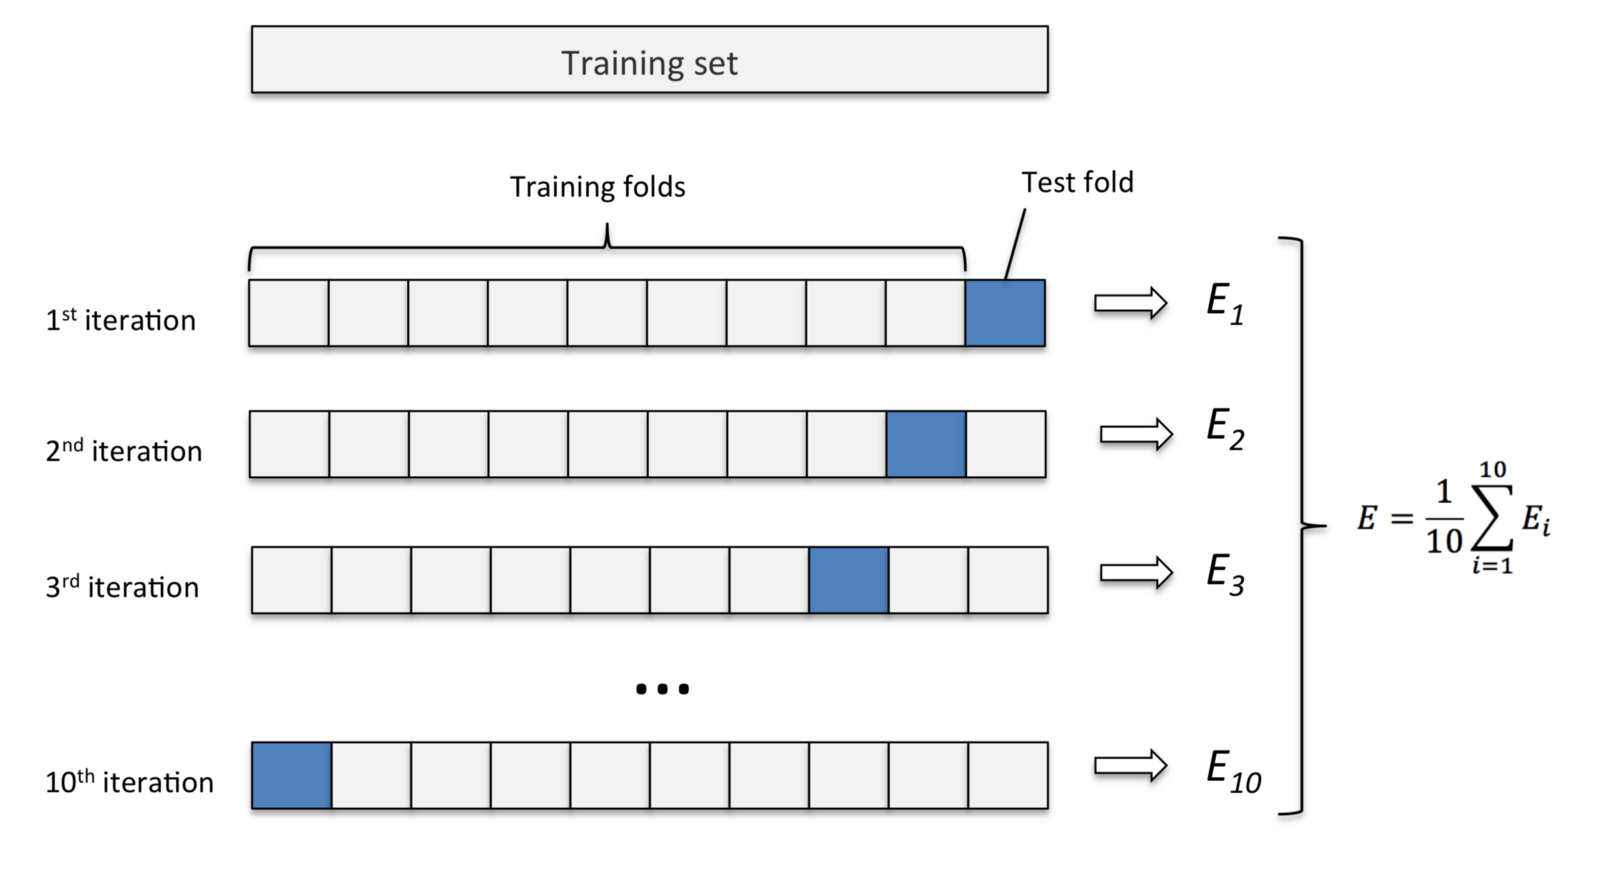
\includegraphics[width=0.8\linewidth]{kfold.png}
	\caption{Wizualizacja działania K-fold dla K=10}
	\label{fig:kfold}
\end{figure}
%obrazek z https://stats.stackexchange.com/questions/336038/question-on-double-cross-validation

\subsubsection{Metodologia oceny skuteczności}

Klasyfikujemy cztery klasy uderzeń serca:
\begin{itemize}
\item Nadkomorowy skurcz dodatkowy (SVEB)
\item Komorowy skurcz dodatkowy (VEB)
\item Uderzenia połączone (F)

\end{itemize}

W celu oceny skuteczności naszych predykcji konieczne było wybranie odpowiednich metryk, które dawałaby informację o jakości testowanych sieci. Ponieważ rozważany problem sprowadza się do klasyfikacji wieloklasowej, niemożliwe było wykorzystanie gotowych metryk dostępnych w bibliotece Keras. Spośród sposobów oceny modeli dla klasyfikacji wieloklasowej \cite{mlpsurvey2010} do eksperymentów wybraliśmy następujące:

\begin{description}
\item [Skuteczność (\emph{Accuracy})] W wypadku jednej klasy jest to stosunek ilości poprawnie sklasyfikowanych przypadków do liczby wszystkich przypadków. Dla klasyfikacji wieloklasowej skuteczność zdefiniowana jest jako średnia skuteczności klasyfikacji dla poszczególnych klas.

\item [Błąd średniokwadratowy (\emph{Mean Squared Error})] Błąd dla pojedynczej próbki jest to odległość między wartością oczekiwaną, a przewidywaną. Metryka ta jest równa średniej kwadratów tych błędów dla wszystkich próbek. Ma to efekt taki, że na błąd mocniej wpływają duże różnice między wartościami. Dla idealnego klasyfikatora błąd byłby równy jeden.

\item [Precyzja (\emph{Precision})] Precyzja dla jednej klasy to stosunek poprawnie sklasyfikowanych wystąpień do wszystkich przewidzianych wystąpień. Dla klasyfikacji wieloklasowej jest to średnia precyzji jednoklasowej ze wszystkich klas. W naszym wypadku jest to średnia stosunku poprawnie przewidzianych arytmii do wszystkich przewidzianych wystąpień.

\item [Czułość (\emph{Recall})] Czułość dla jednej klasy to stosunek poprawnie przewidzianych pozytywów do ilości pozytywnych próbek. Podobnie jak w przypadku czułości, dla klasyfikacji wieloklasowej jest to średnia metryki jednoklasowej ze wszystkich klas. Dla naszego problemu jest to średnia stosunku poprawnie przewidzianych wystąpień do wszystkich arytmii.

\item [Miara $F_1$ (\emph{$F_1$-Measure})] Jest to średnia harmoniczna czułości i precyzji, dzięki czemu jej wartość dokładniej odzwierciedla jakość klasyfikatora niż osobne metryki.
\end{description}


\subsubsection{Wyniki dla różnych modeli}

Przy obrabianiu wyników poszczególnych sieci bardzo przydatne okazało się narzędzie Jupyter Notebook.
\begin{figure}[H]
	\centering
	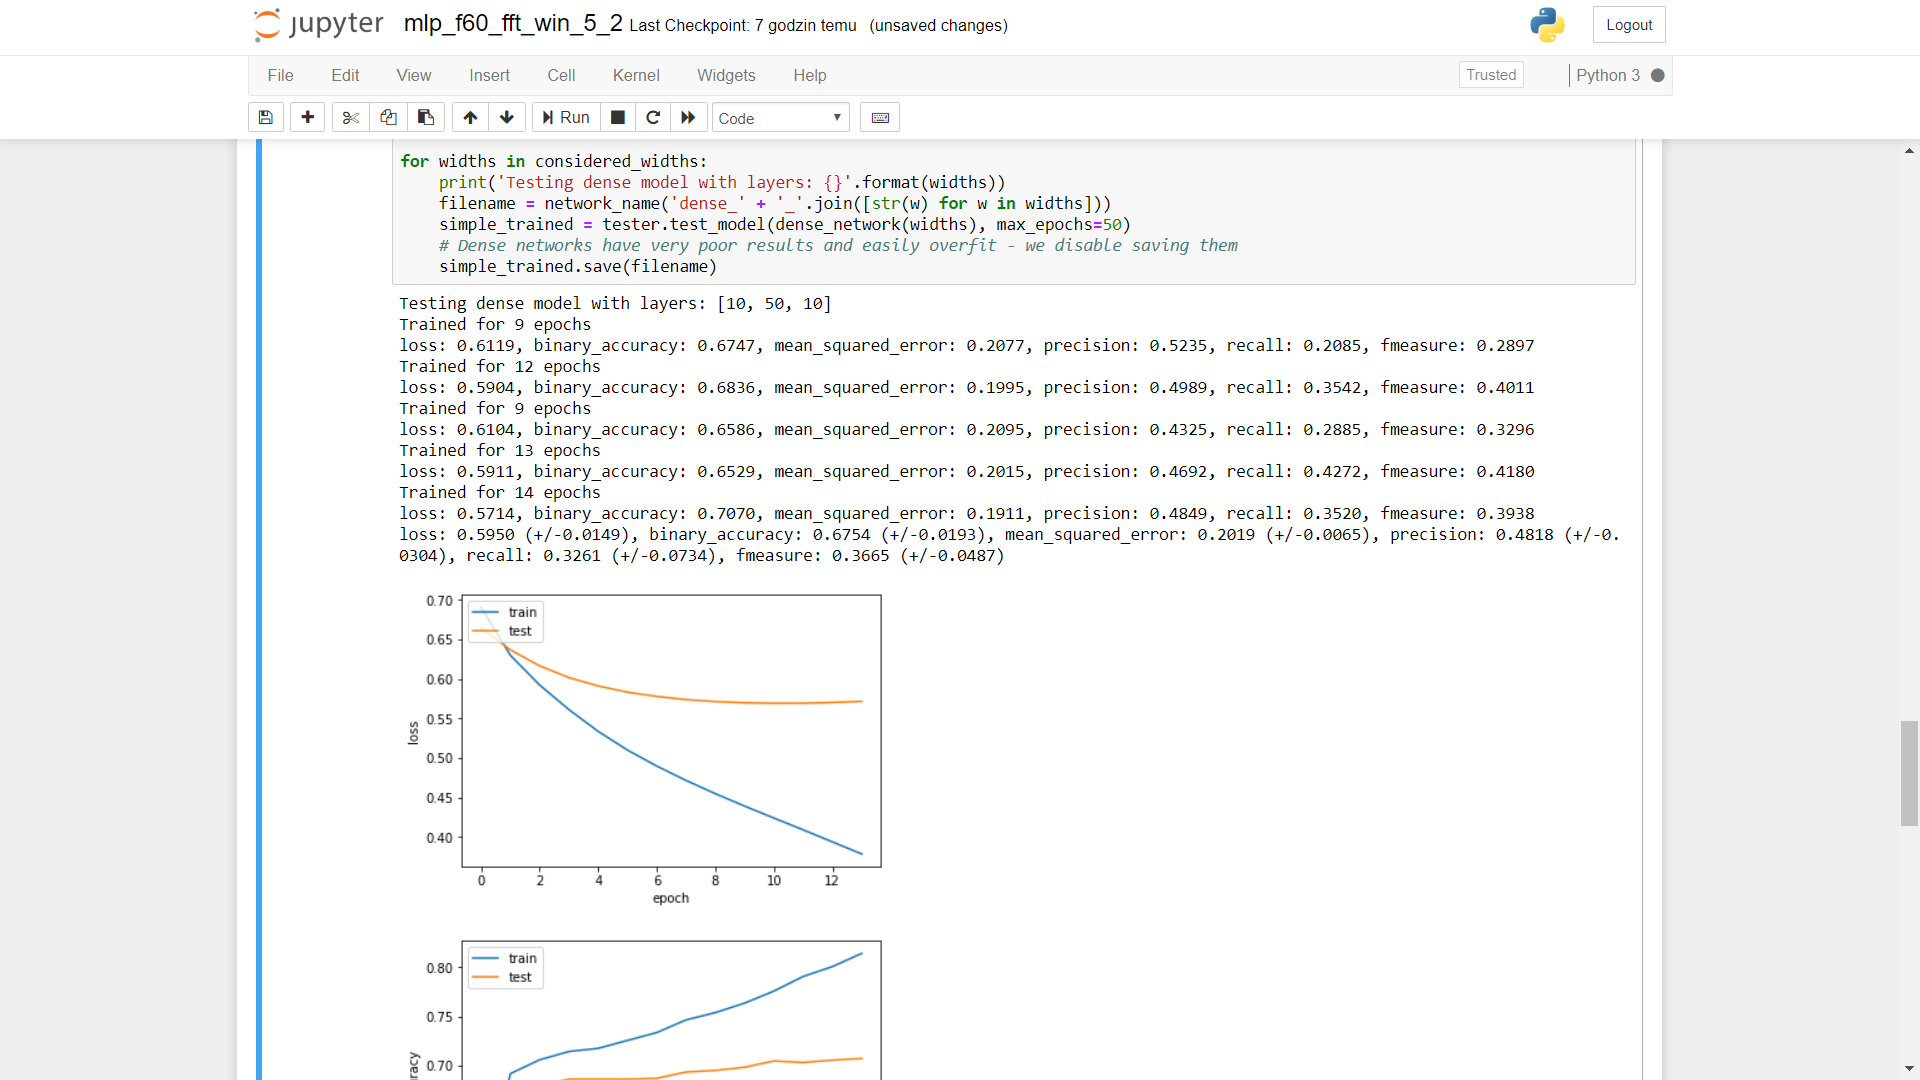
\includegraphics[width=0.7\linewidth]{jupyter.png}
	\caption{Widok z notebooka Jupytera}
	\label{fig:jupyter}
\end{figure}

\paragraph{Sieci gęste} - wyniki dla sieci gęstych składających się z kilku warstw ukrytych o różnych rozmiarach oraz warstwy wyjściowej.

Sieć gęsta z 3 warstwami ukrytymi o szerokościach 10, 50 i 10.

\begin{lstlisting}[float=h!, style=result, caption={Wyniki sieci gęstej o rozmiarach warstw 10, 50, 10}]
loss: 0.6130 (+/-0.0159), binary_accuracy: 0.6704 (+/-0.0213), mean_squared_error: 0.2102 (+/-0.0071), precision: 0.4789 (+/-0.0475), recall: 0.3681 (+/-0.0560), fmeasure: 0.3917 (+/-0.0182)
\end{lstlisting}

\begin{figure}[H]
	\centering
	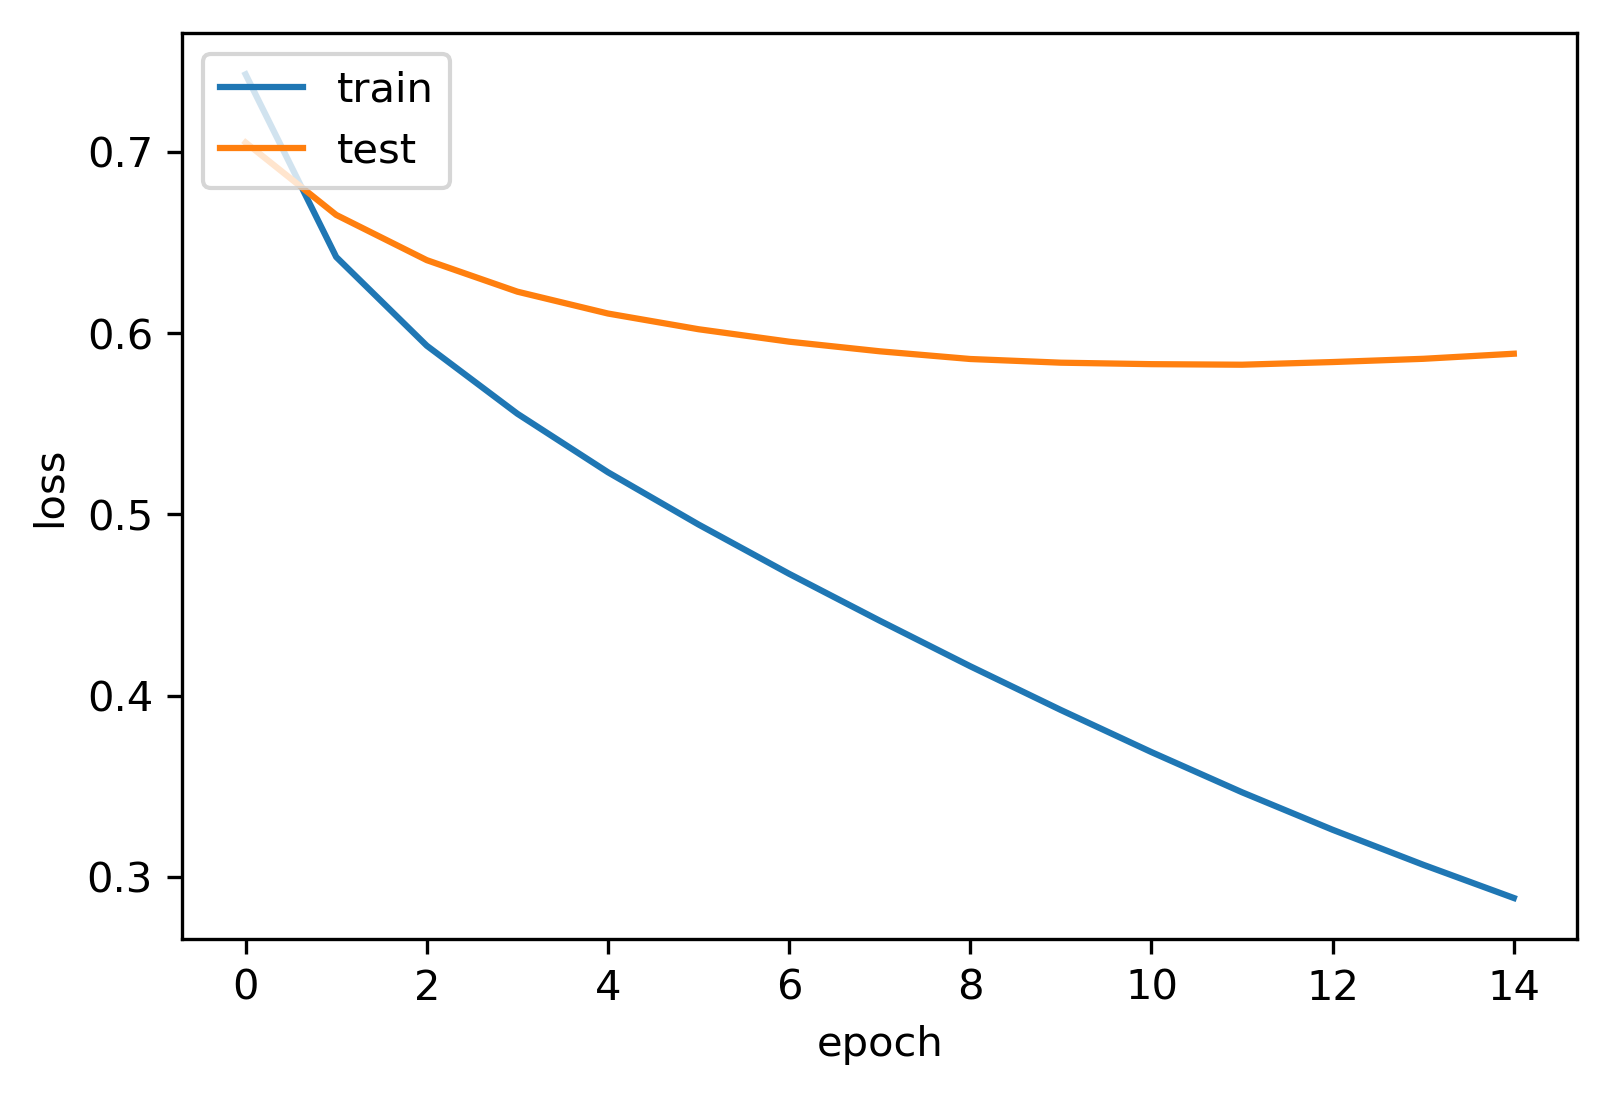
\includegraphics[width=0.7\linewidth]{dense_10_50_10_loss.png}
	\caption{Wykres straty dla sieci gęstej o rozmiarach warstw 10, 50, 10}
	\label{fig:dense_10_50_10_loss}
\end{figure}
\begin{figure}[H]
	\centering
	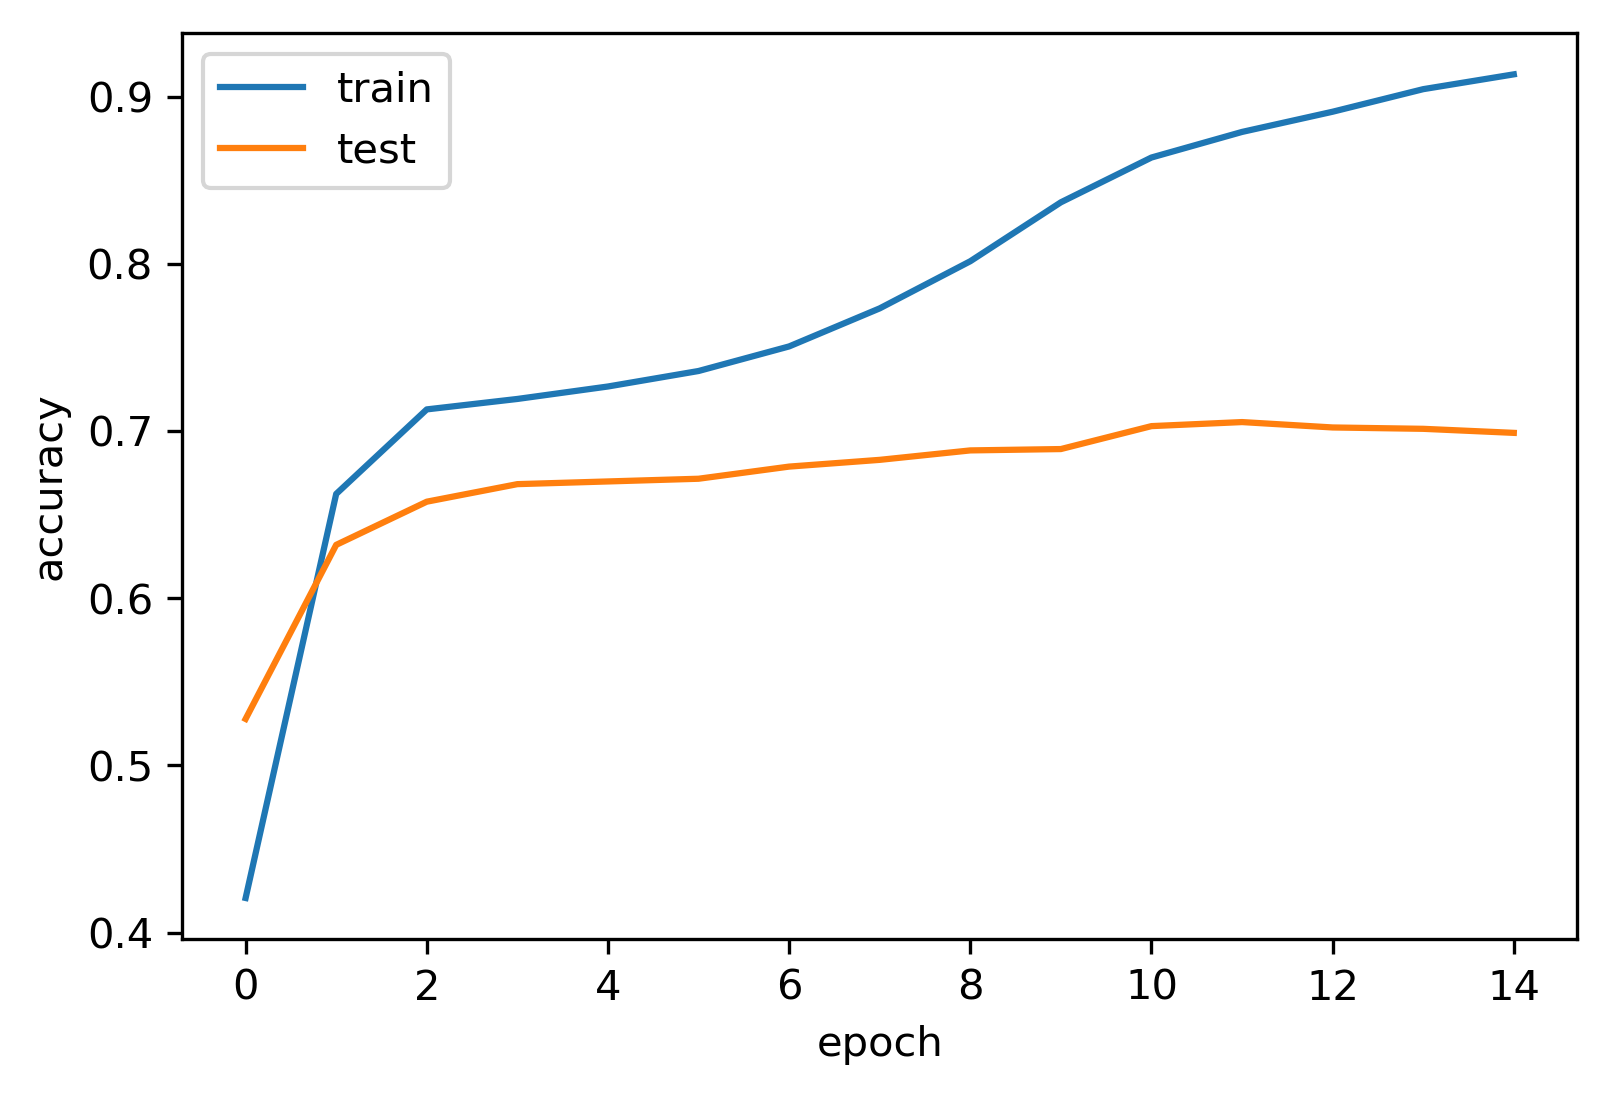
\includegraphics[width=0.7\linewidth]{dense_10_50_10_acc.png}
	\caption{Wykres dokładności dla sieci gęstej o rozmiarach warstw 10, 50, 10}
	\label{fig:dense_10_50_10_acc}
\end{figure}

Sieć gęsta z 2 warstwami ukrytymi o szerokości 100 i 100.

\begin{lstlisting}[float=h!, style=result, caption={Wyniki sieci gęstej o rozmiarach warstw 100, 100}]
loss: 0.6172 (+/-0.0219), binary_accuracy: 0.6820 (+/-0.0200), mean_squared_error: 0.2086 (+/-0.0084), precision: 0.4631 (+/-0.0315), recall: 0.3754 (+/-0.0372), fmeasure: 0.3973 (+/-0.0376)
\end{lstlisting}

\begin{figure}[H]
	\centering
	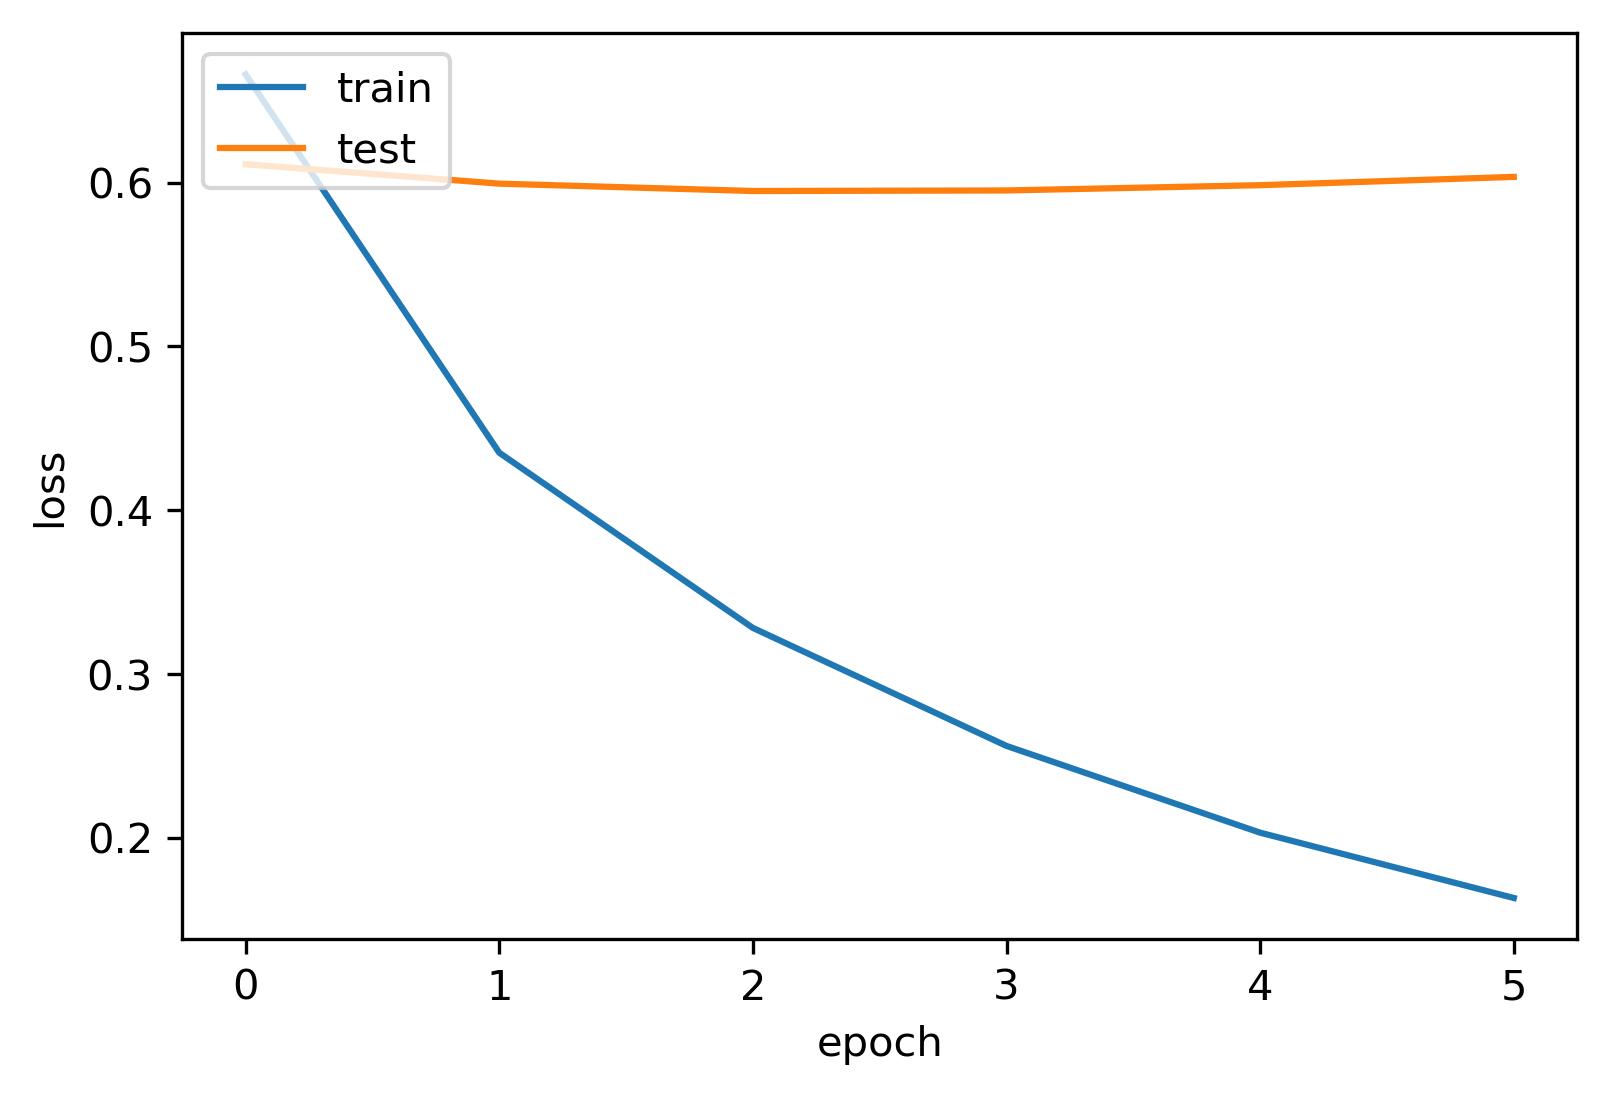
\includegraphics[width=0.7\linewidth]{dense_100_100_loss.png}
	\caption{Wykres straty dla sieci gęstej o rozmiarach warstw 100, 100}
	\label{fig:dense_100_100_loss}
\end{figure}
\begin{figure}[H]
	\centering
	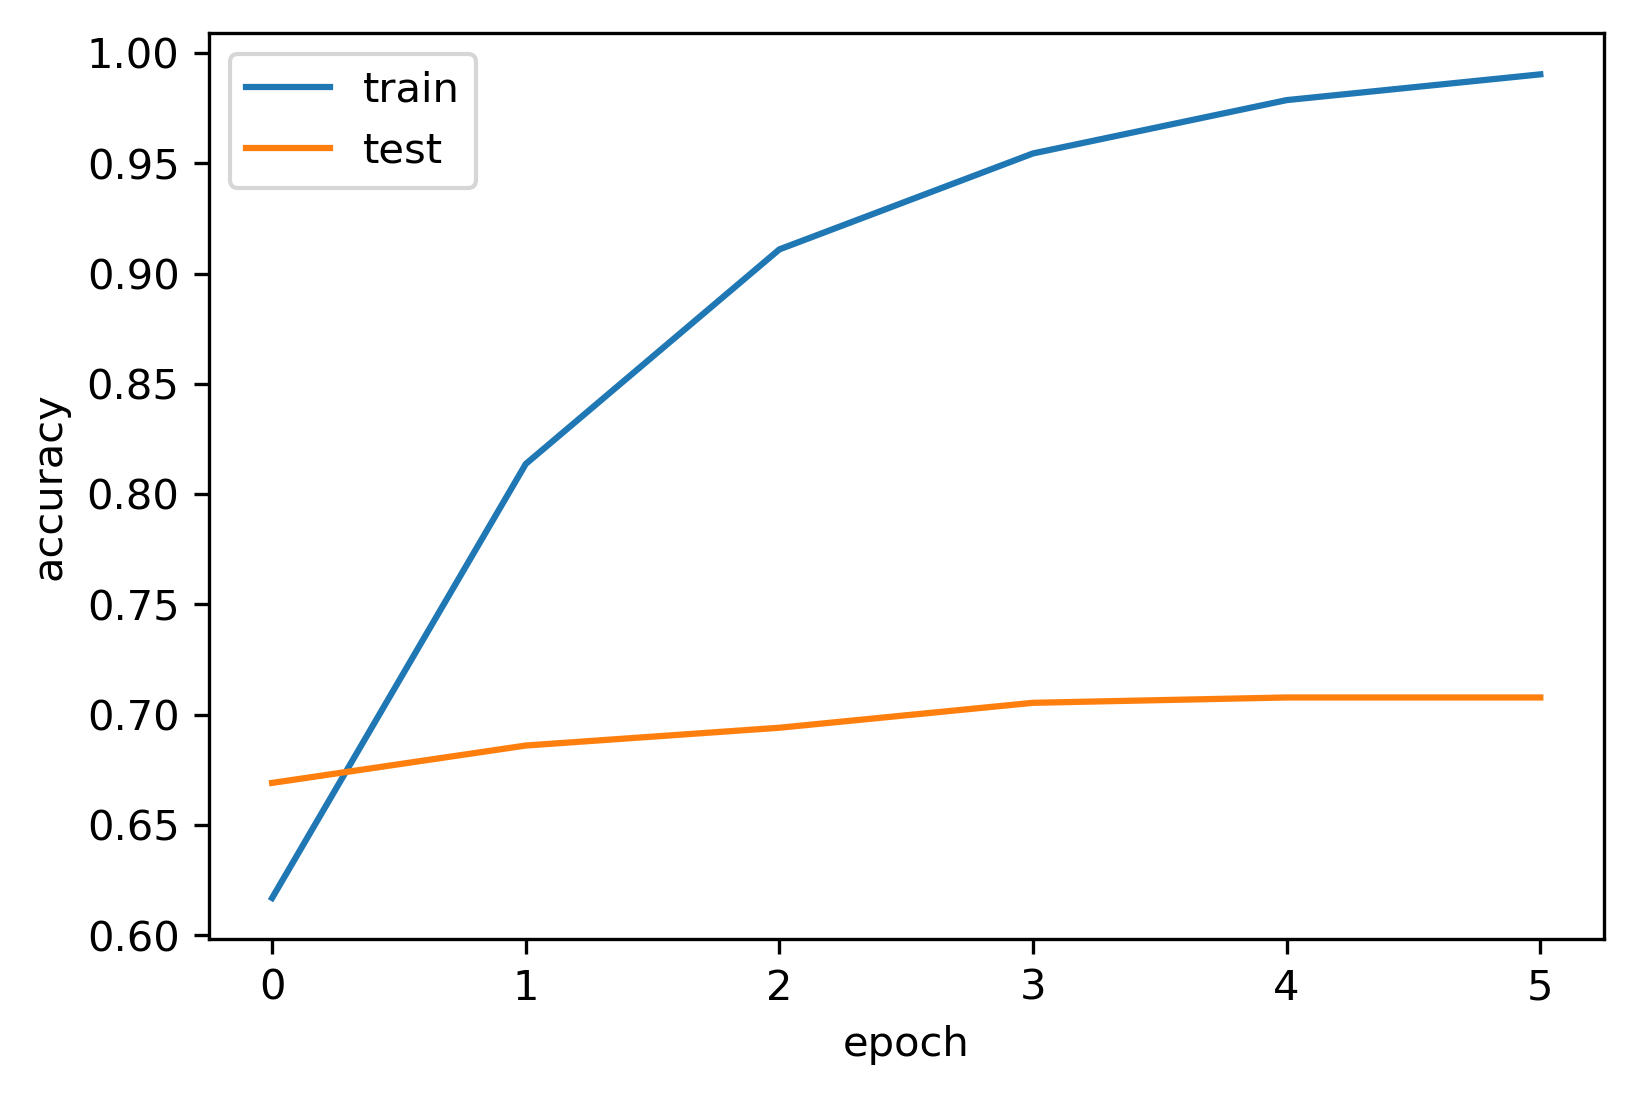
\includegraphics[width=0.7\linewidth]{dense_100_100_acc.png}
	\caption{Wykres dokładności dla sieci gęstej o rozmiarach warstw 100, 100}
	\label{fig:dense_100_100_acc}
\end{figure}

Sieć gęsta z 3 warstwami  ukrytymi o szerokościach 100, 200 i 100.

\begin{lstlisting}[float=h!, style=result, caption={Wyniki sieci gęstej o rozmiarach warstw 100, 200, 100}]
loss: 0.5799 (+/-0.0133), binary_accuracy: 0.6900 (+/-0.0091), mean_squared_error: 0.1969 (+/-0.0045), precision: 0.4926 (+/-0.0249), recall: 0.3370 (+/-0.0282), fmeasure: 0.3836 (+/-0.0115)
\end{lstlisting}

\begin{figure}[H]
	\centering
	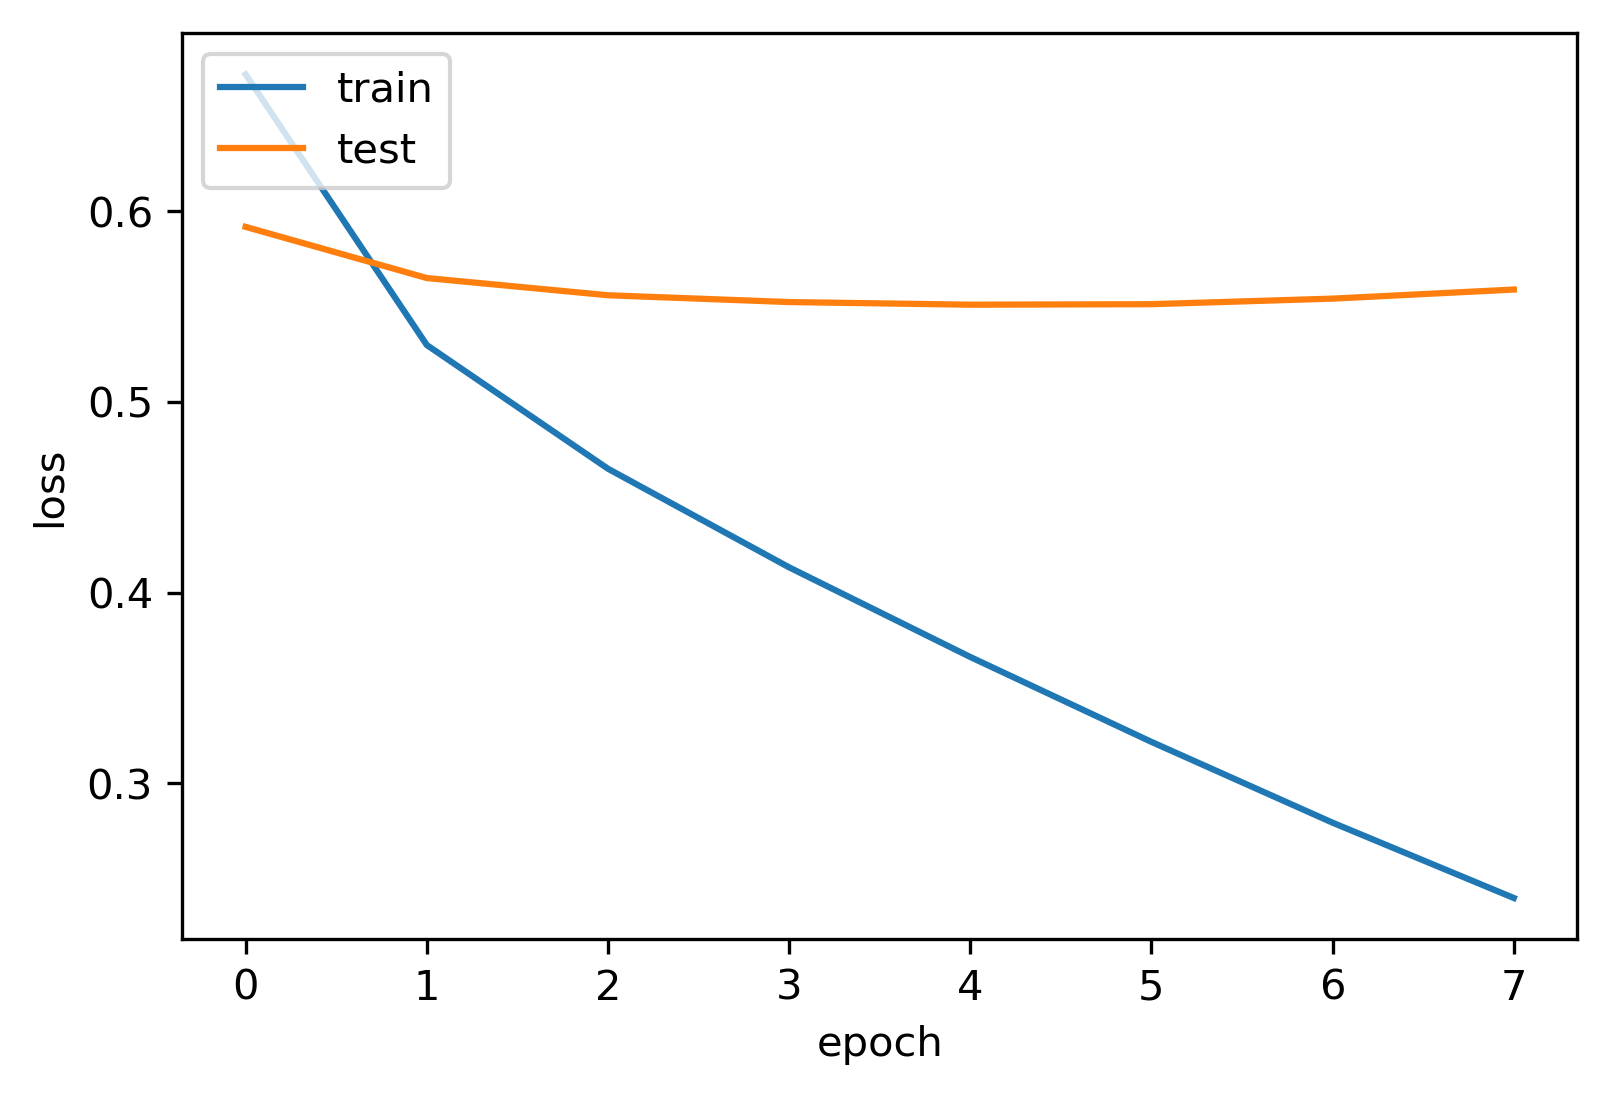
\includegraphics[width=0.7\linewidth]{dense_100_200_100_loss.png}
	\caption{Wykres straty dla sieci gęstej o rozmiarach warstw 100, 200, 100}
	\label{fig:dense_100_200_100_loss}
\end{figure}
\begin{figure}[H]
	\centering
	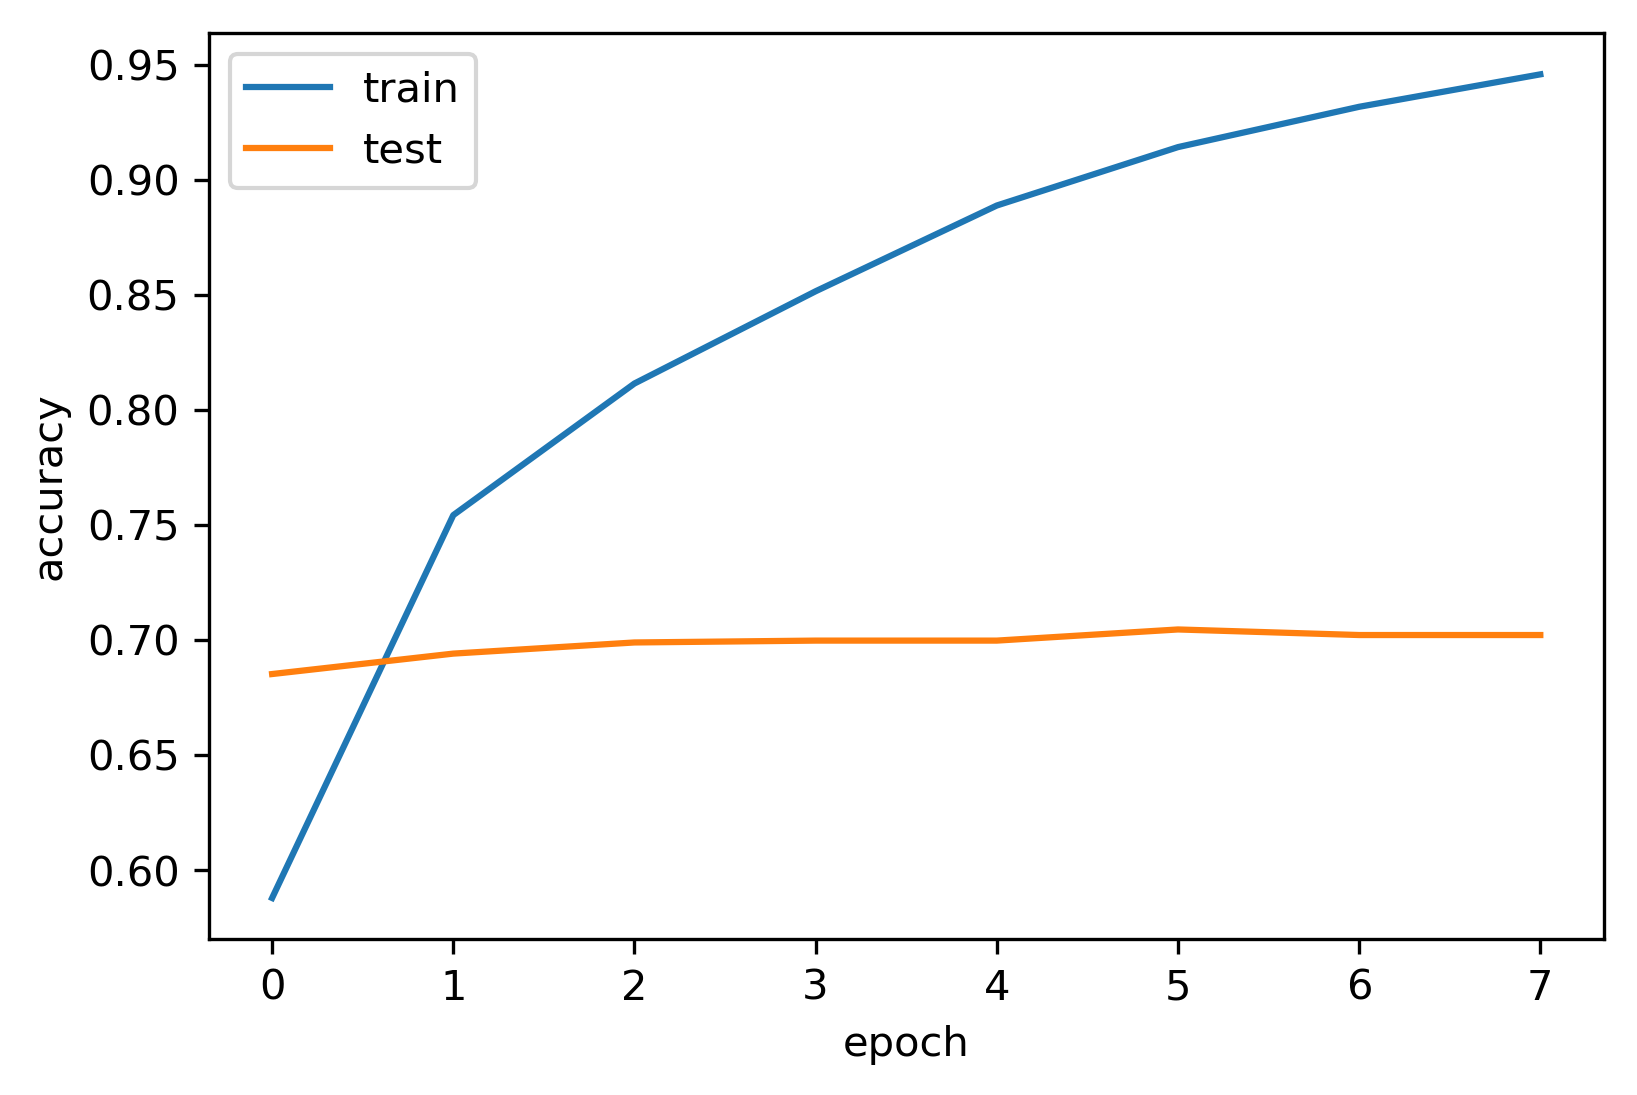
\includegraphics[width=0.7\linewidth]{dense_100_200_100_acc.png}
	\caption{Wykres dokładności dla sieci gęstej o rozmiarach warstw 100, 200, 100}
	\label{fig:dense_100_200_100_acc}
\end{figure}

\paragraph{Sieci konwolucyjne} - sieci konwolucyje %TODO KD opisy

Sieć konwolucyjna pool=16, warstwy=[(4, 16), (16, 16)]

\begin{lstlisting}[float=h!, style=result, caption={Wyniki sieci konwolucyjnej}]
loss: 0.3686 (+/-0.0243), binary_accuracy: 0.8382 (+/-0.0234), mean_squared_error: 0.1174 (+/-0.0095), precision: 0.8013 (+/-0.0821), recall: 0.6223 (+/-0.1151), fmeasure: 0.6768 (+/-0.0526)
\end{lstlisting}

\begin{figure}[H]
	\centering
	\captionsetup{justification=centering}
	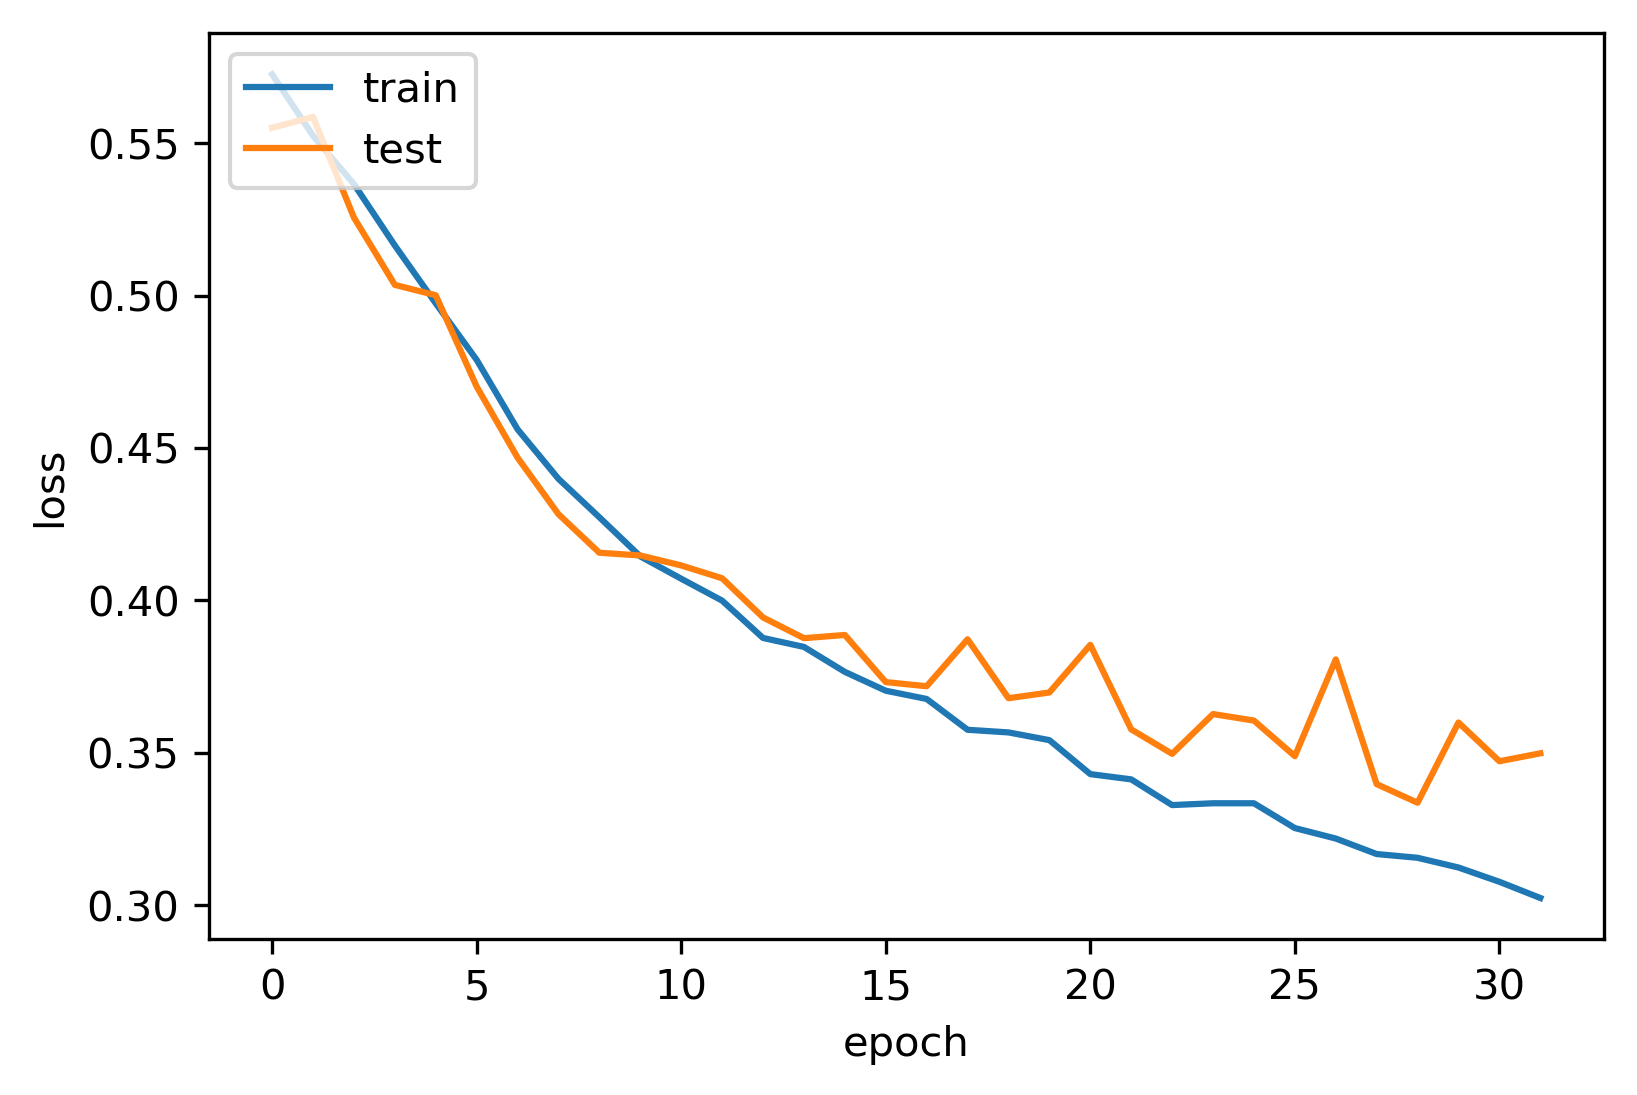
\includegraphics[width=0.7\linewidth]{conv_16_4_loss.png}
	\caption{Wykres straty dla sieci konwolucyjnej z parametrami: pool=16, warstwy=[(4, 16), (16, 16)]}
	\label{fig:conv_16_4_loss}
\end{figure}
\begin{figure}[H]
	\centering
	\captionsetup{justification=centering}
	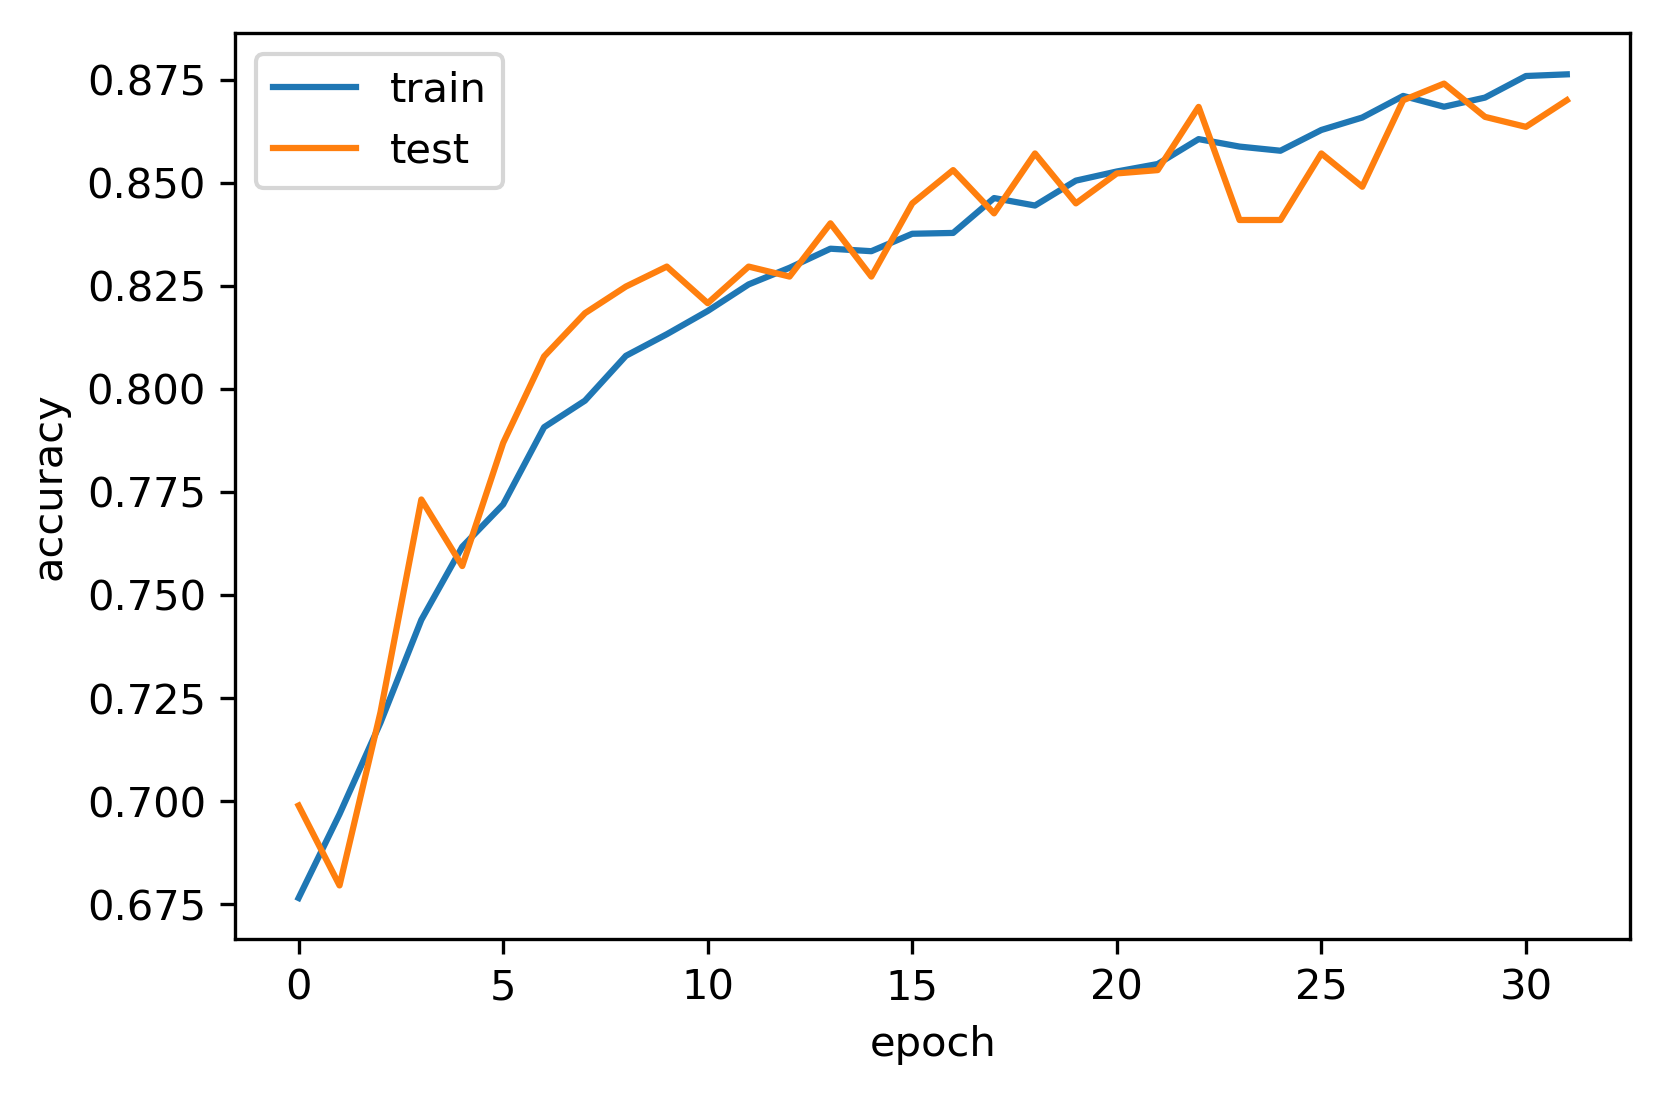
\includegraphics[width=0.7\linewidth]{conv_16_4_acc.png}
	\caption{Wykres dokładności dla sieci konwolucyjnej z parametrami: pool=16, warstwy=[(4, 16), (16, 16)]}
	\label{fig:conv_16_4_acc}
\end{figure}

Sieć konwolucyjna pool=16, warstwy=[(32, 16), (16, 16)]

\begin{lstlisting}[float=h!, style=result, caption={Wyniki sieci konwolucyjnej}]
loss: 0.3688 (+/-0.0522), binary_accuracy: 0.8294 (+/-0.0351), mean_squared_error: 0.1178 (+/-0.0204), precision: 0.7980 (+/-0.1436), recall: 0.6589 (+/-0.1287), fmeasure: 0.6813 (+/-0.0438)
\end{lstlisting}

\begin{figure}[H]
	\centering
	\captionsetup{justification=centering}
	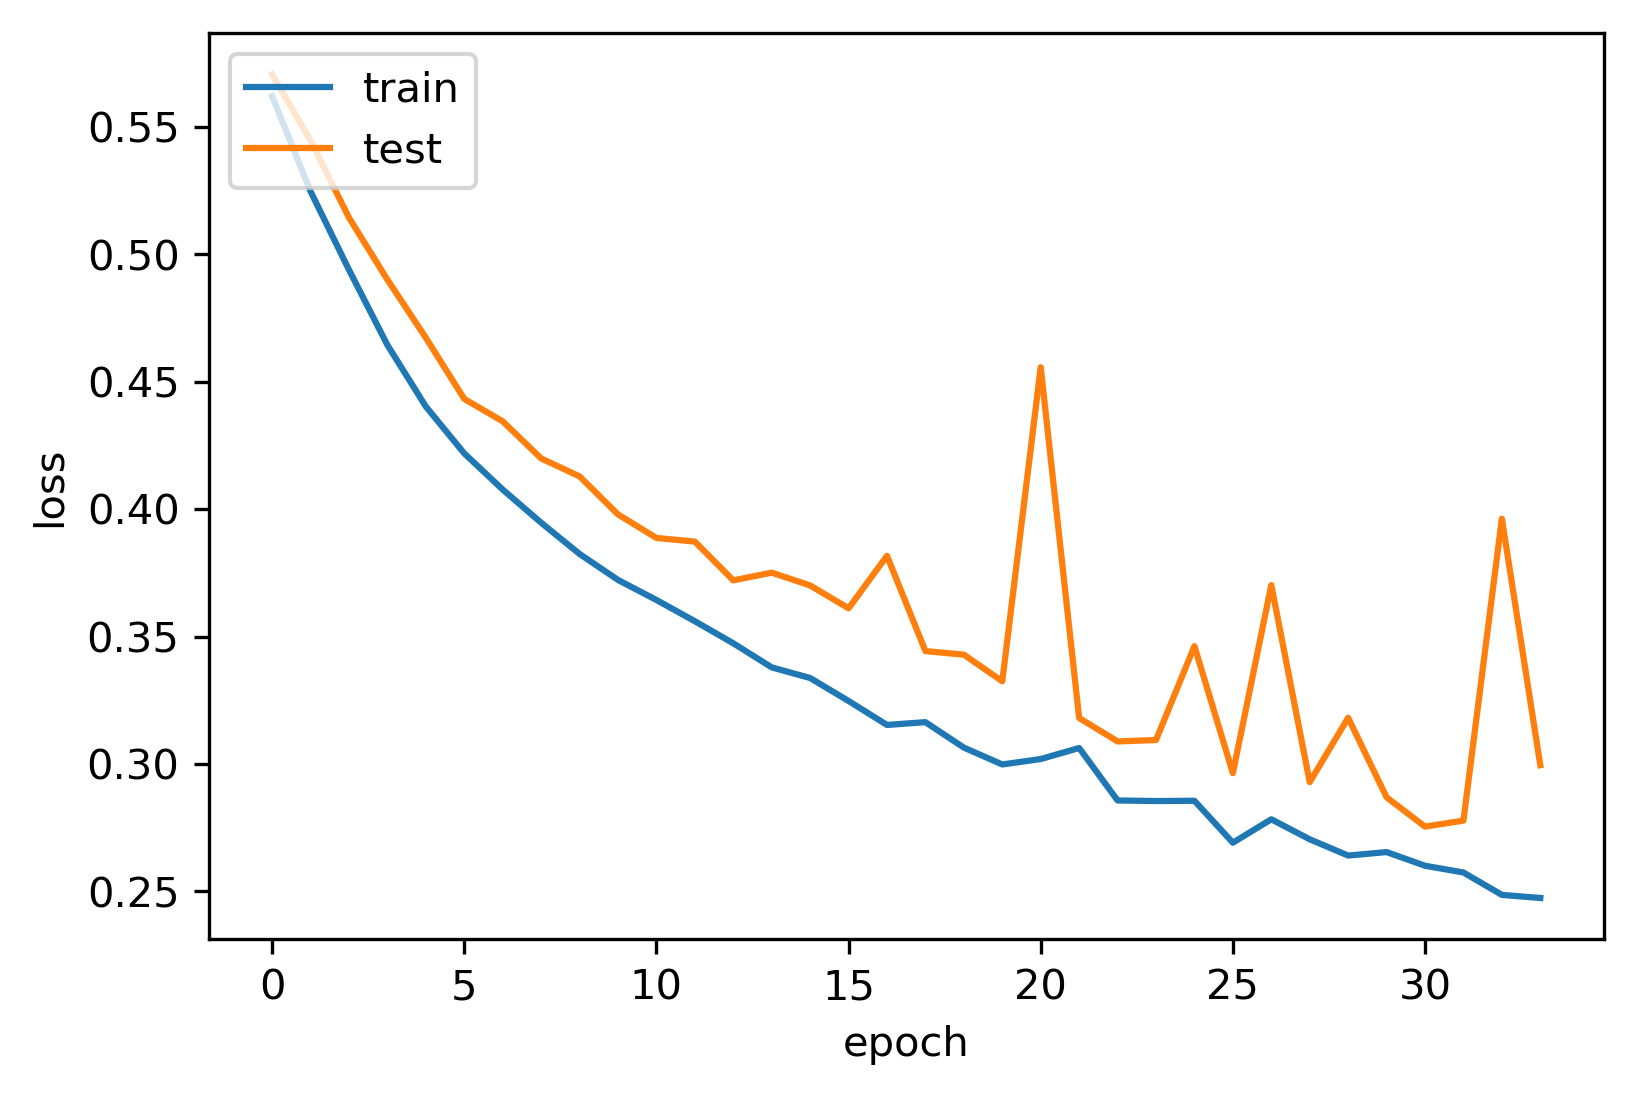
\includegraphics[width=0.7\linewidth]{conv_16_32_loss.png}
	\caption{Wykres straty dla sieci konwolucyjnej z parametrami: pool=16, warstwy=[(32, 16), (16, 16)]}
	\label{fig:conv_16_32_loss}
\end{figure}
\begin{figure}[H]
	\centering
	\captionsetup{justification=centering}
	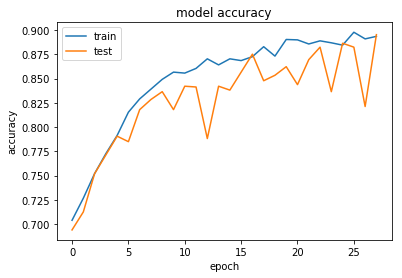
\includegraphics[width=0.7\linewidth]{conv_16_32_acc.png}
	\caption{Wykres dokładności dla sieci konwolucyjnej z parametrami: pool=16, warstwy=[(32, 16), (16, 16)]}
	\label{fig:conv_16_32_acc}
\end{figure}

Sieć konwolucyjna pool=8, warstwy=[(16, 16), (8, 16), (4, 16)]

\begin{lstlisting}[float=h!, style=result, caption={Wyniki sieci konwolucyjnej}]
loss: 0.3577 (+/-0.0553), binary_accuracy: 0.8421 (+/-0.0366), mean_squared_error: 0.1134 (+/-0.0218), precision: 0.8229 (+/-0.0607), recall: 0.5770 (+/-0.0925), fmeasure: 0.6546 (+/-0.0808)
\end{lstlisting}

\begin{figure}[H]
	\centering
	\captionsetup{justification=centering}
	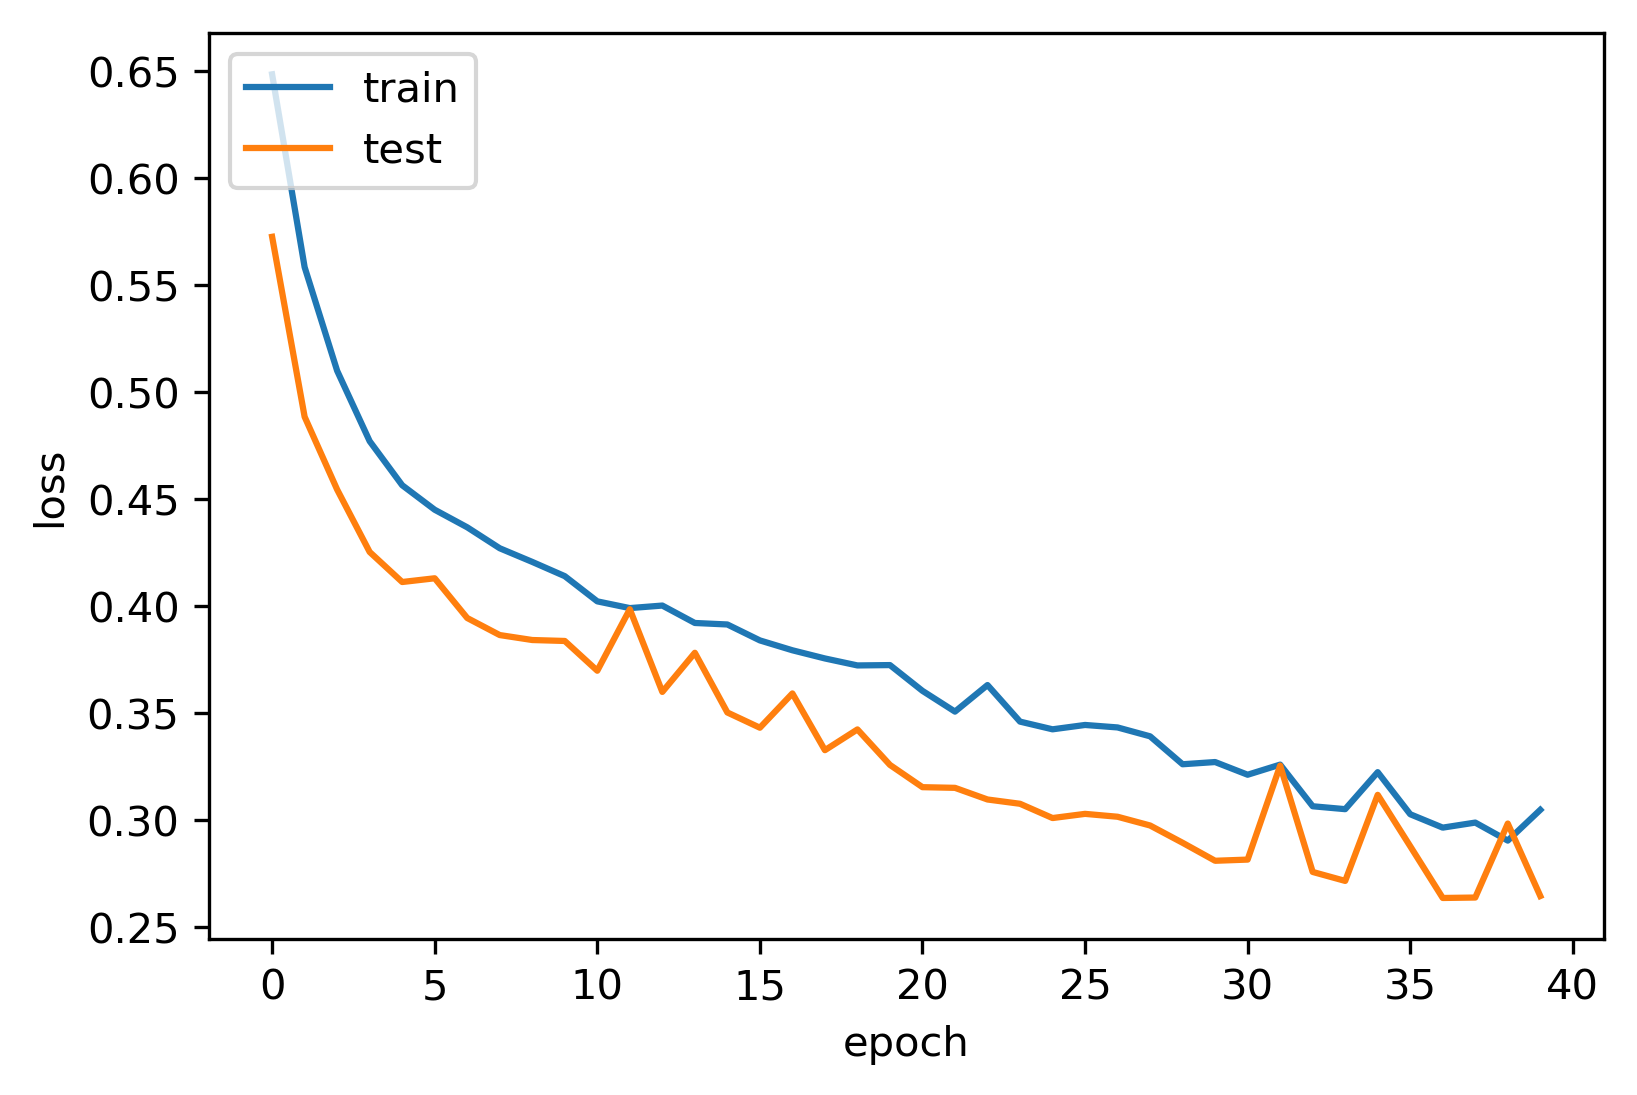
\includegraphics[width=0.7\linewidth]{conv_8_16_loss.png}
	\caption{Wykres straty dla sieci konwolucyjnej z parametrami: pool=8, warstwy=[(16, 16), (8, 16), (4, 16)]}
	\label{fig:conv_8_16_loss}
\end{figure}
\begin{figure}[H]
	\centering
	\captionsetup{justification=centering}
	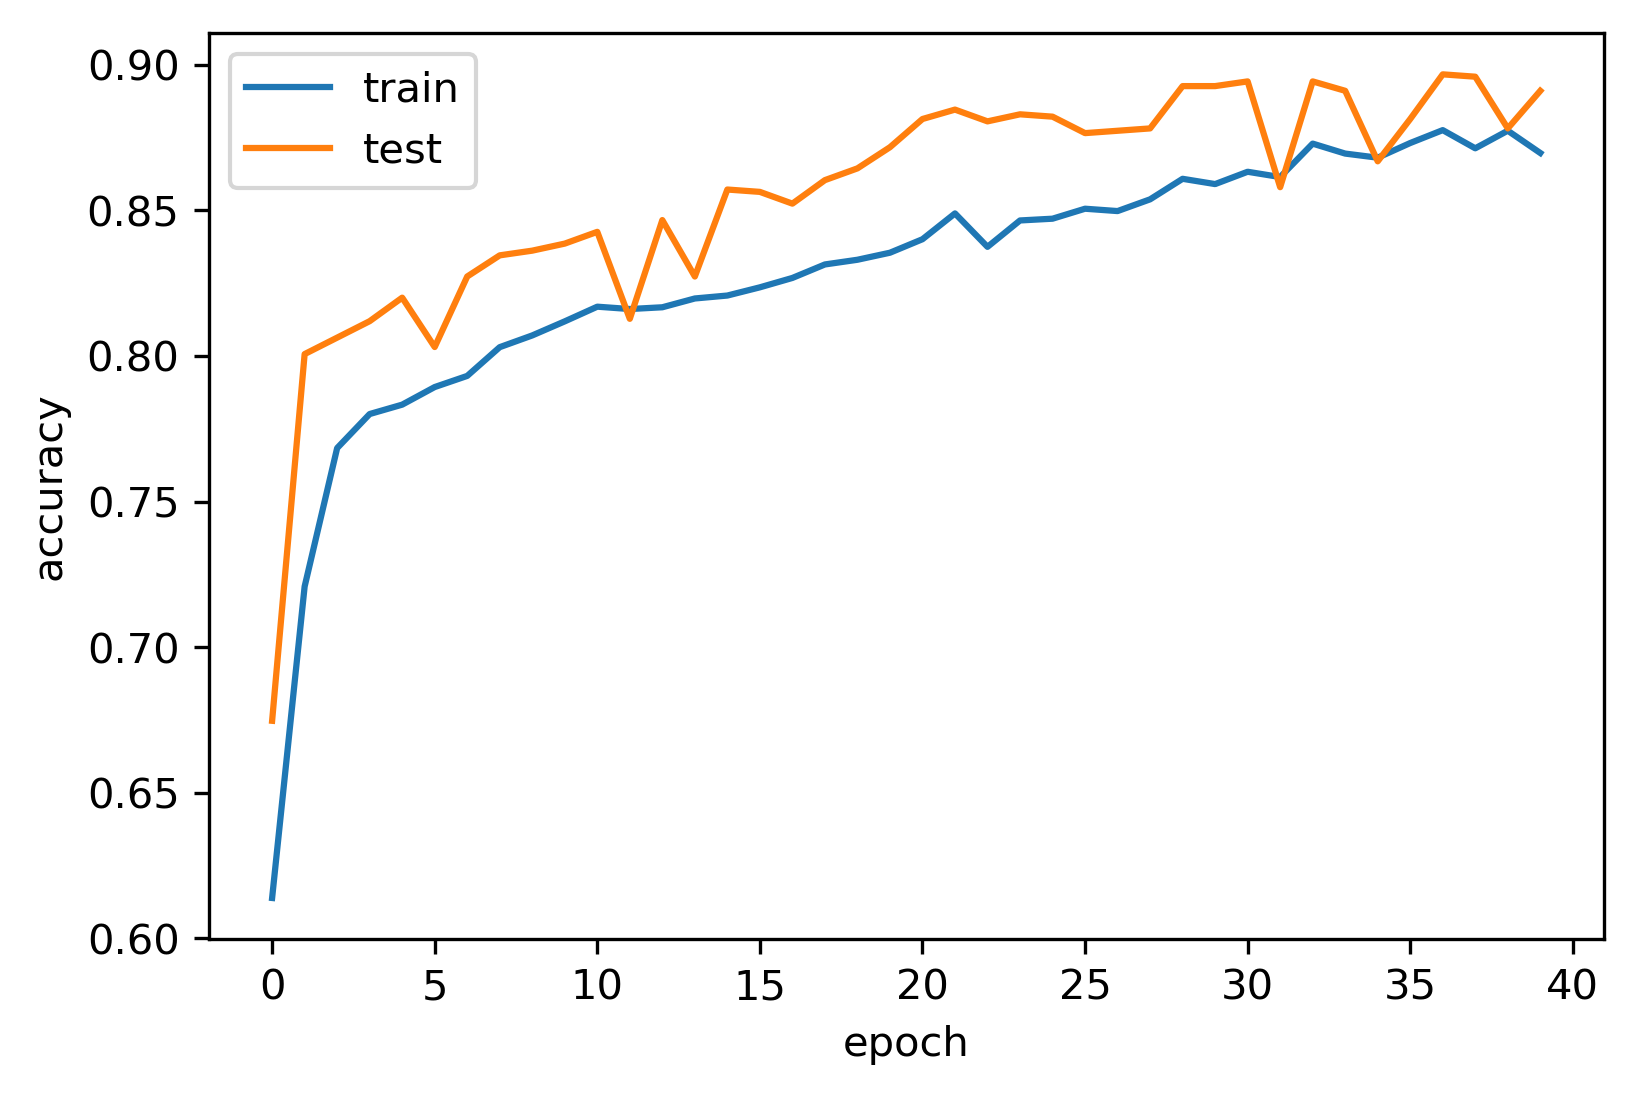
\includegraphics[width=0.7\linewidth]{conv_8_16_acc.png}
	\caption{Wykres dokładności dla sieci konwolucyjnej z parametrami: pool=8, warstwy[(16, 16), (8, 16), (4, 16)]}
	\label{fig:conv_8_16_acc}
\end{figure}


\subsection{Testy}

Wraz z rozrastaniem się projektu staraliśmy się równolegle pisać testy dla nowo powstających elementów. Ułatwiło to znacznie znajdowanie błędów i usprawniło tworzenie projektu.
%TODO 
\begin{lstlisting}[float=h!, caption={Przykładowy test interfejsu}]
def test_loading_and_plotting_predict(qtbot, manager):
    """
    Simple test for loading and plotting in predict window
    """
    predict = manager.predict
    predict.load_plot_from_file("100.dat")
    predict.set_new_plot()

    assert predict.start == 0
    assert predict.start_line.text() == "0"
    assert predict.sig_len > 0
    assert predict.figure is not None
\end{lstlisting}

\begin{lstlisting}[float=h!, caption={Przykładowy test normalizacji}]
def test_standard_normalizer():
    # Given:
    # Create random sequence of uniform values from interval [0, 1)
    length = 100
    random_uniform = np.random.rand(length)
    # Create the normalizer to test
    normalizer = StandardNormalizer()
    # Helper pipe to save the result
    result = None

    def set_result(v):
        nonlocal result
        result = v

    endp = FunctionLayer(set_result)
    # Connect normalizer to ending pipe
    normalizer.set_next(endp)

    # When:
    normalizer.push_value(random_uniform)

    # Then:
    # Length of output sequence should be the same as input sequence
    assert len(result) == length
    # Mean should be zero
    assert abs(result.mean()) < epsilon
    # Standard deviation should be zero
    assert abs(result.std() - 1.0) < epsilon
\end{lstlisting}

\section{\SectionTitleWorkOrganization}
\label{sec:organizacja-pracy}
%\emph{Struktura zespołu (role poszczególnych osób), krótki opis i
%  uzasadnienie przyjętej metodyki i/lub kolejności prac, planowane i
%  zrealizowane etapy prac ze wskazaniem udziału poszczególnych
%  członków zespołu, wykorzystane praktyki i narzędzia w zarządzaniu
%  projektem.}

\subsection{Charakterystyka projektu}

Zaproponowany temat projektu obejmował zagadnienia z dziedziny nie powiązanej z naszym kierunkiem studiów. Praca ma też w pewnym stopniu charakter eksperymentalny, gdyż nie jest udokumentowane w jakim stopniu metody uczenia maszynowego mają zastosowanie w predykcji arytmii serca na podstawie samego wykresu EKG. Wiele czasu poświęciliśmy na testowanie skuteczności predykcji różnych modeli sieci. Dodatkowo musieliśmy też zbadać wpływ parametrów danych wejściowych, takich jak długość fragmentu EKG na wejściu, okres w którym staramy się przewidzieć wystąpienie arytmii, jak i stopień redukcji szumów czy interpolacja danych do mniejszych częstotliwości. 

Dodatkowo aby predykcja była możliwa musimy mieć oznaczone dane treningowe, na których będziemy mogli trenować naszą sieć. Jednak ciężko znaleźć ogólnodostępne dane, które spełniałyby to wymaganie. Wykorzystaliśmy więc jedynie bazę, którą zaproponował nam promotor. Ze względu na nieduży rozmiar danych, staraliśmy się w pełni wykorzystać używaną przez nas bazę danych.

\subsection{Struktura zespołu i role}

W skład naszego zespołu wchodziło dwóch studentów Informatyki. Pracę nad systemem podzieliliśmy na zadania, które staraliśmy się równo podzielić między członkami zespołu. Dodatkowo przy dzieleniu się pracą braliśmy pod uwagę umiejętności, zainteresowania i doświadczenie. Nad szczególnymi i kluczowymi elementami projektu pracowaliśmy wspólnie.

\begin{itemize}
	\item \textbf{Tomasz Nizio}	
	
	Implementacja redukcja szumów o niskich częstotliwościach przy pomocy FFT, projekt całego interfejsu graficznego, przełączanie pomiędzy widokami, rysowanie wykresu EKG oraz nawigacja po nim, wyświetlanie wyników oraz logów predykcji
	\item  \textbf{Konrad Dobroś}
	
	Implementacja pobierania bazy z sieci, wczytywania, interpolacji oraz normalizacji danych, podział danych na treningowe i testowe, struktura silnika predykcji, testowanie różnych modeli siec neuronowych, dobór parametrów wejścia
	
\end{itemize}

Wspólnie zajmowaliśmy się wyszukiwaniem informacji przydatnych w rozwoju projektu, tworzeniem prymitywnego prototypu, pisaniem testów dla elementów które stworzyliśmy, a także tworzeniem dokumentacji.
Dodatkowo za każdym razem recenzowaliśmy się nawzajem w sprawie wprowadzanych zmian.

\subsection{Etapy przebiegu pracy}

Prace nad projektem przebiegały dosyć nieregularnie. Pod koniec semestru letniego udało się uzyskać prototyp o minimalnej funkcjonalności. W trakcie przerwy semestralnej prace nad projektem spowolniły. Największa część projektu powstała w trakcie semestru zimowego. 

Wyszczególnić możemy następujące etapy prac:

\subsubsection{Zapoznanie z tematyką projektu oraz konfiguracja środowiska}

Czas trwania: 03.2018 - 04.2018
\newline
Osiągnięte cele:
\begin{itemize}
	\item zapoznanie się z pojęciem arytmii, na czym polega, jak można ją wykrywać
	\item zapoznanie się z postacią wykresu EKG, co dokładnie przedstawia
	\item zapoznanie się z działaniem sieci neuronowych oraz jak można ją wykorzystać do przewidywania wystąpienia arytmii
	\item utworzenie środowiska - repozytorium, CI, narzędzia organizacji pracy
	\item research technologii
\end{itemize}

\subsubsection{Zintegrowanie bazy danych}

Czas trwania: 04.2018 - 05.2018
\newline
Osiągnięte cele:
\begin{itemize}
	\item zapoznanie się ze strukturą wykorzystywanej bazy EKG
	\item pobranie bazy danych
	\item wyodrębnienie wymaganych danych z bazy
\end{itemize}

\subsubsection{Stworzenie prototypu}

Czas trwania: 05.2018 - 06.2018
\newline
Osiągnięte cele:
\begin{itemize}
	\item stworzenie prostego modelu sieci
	\item określenie formatu danych na wejściu sieci neuronowej
	\item implementacja podstawowych operacji na danych
	\item przygotowanie danych dla takiego modelu
	\item przetestowanie działania przygotowanej sieci
\end{itemize}

\subsubsection{Struktura projektu oraz interfejsu}

Czas trwania: 07.2018 - 09.2018
\newline
Osiągnięte cele:
\begin{itemize}
	\item wyodrębnienie w projekcie poszczególnych modułów
	\item określenie architektury modelu predykcji
	\item wstępny projekt interfejsu graficznego
\end{itemize}

\subsubsection{Implementacja interfejsu oraz testy innych modeli sieci}

Czas trwania: 09.2018 - 10.2018
\newline
Osiągnięte cele:
\begin{itemize}
	\item implementacja podstawowego interfejsu graficznego
	\item redukcja szumów o niskich częstotliwościach na przebiegu EKG
	\item stworzenie bardziej rozbudowanego modelu sieci neuronowej
	\item testy skuteczności predykcji z różnymi parametrami
\end{itemize}

\subsubsection{Połączenie interfejsu z silnikiem predykcji}

Czas trwania: 10.2018 - 11.2018
\newline
Osiągnięte cele:
\begin{itemize}
	\item integracja modelu z interfejsem
	\item wytrenowanie ostatecznych sieci neuronowych
	\item dodanie informacji o arytmiach
\end{itemize}

\subsubsection{Poprawki oraz dokumentacja}

Czas trwania: 11.2018 - 12.2018
\newline
Osiągnięte cele:
\begin{itemize}
	\item poprawki interfejsu
	\item poprawki modelu
	\item stworzenie dokumentacji
\end{itemize}

\subsection{Wykorzystane narzędzia}

Do zarządzania poszczególnymi zadaniami i całym projektem wykorzystaliśmy aplikacje webową \textbf{Trello}. Do komunikacji w zespole wykorzystywaliśmy komunikator \textbf{Slack}, którego zintegrowaliśmy z narzędziem \textbf{GitHub} co sprawiło że na kanał wysyłane były informacje o zmianach w repozytorium. Sporadycznie komunikowaliśmy się również przez \textbf{Skype}.

\begin{figure}[H]
	\centering
	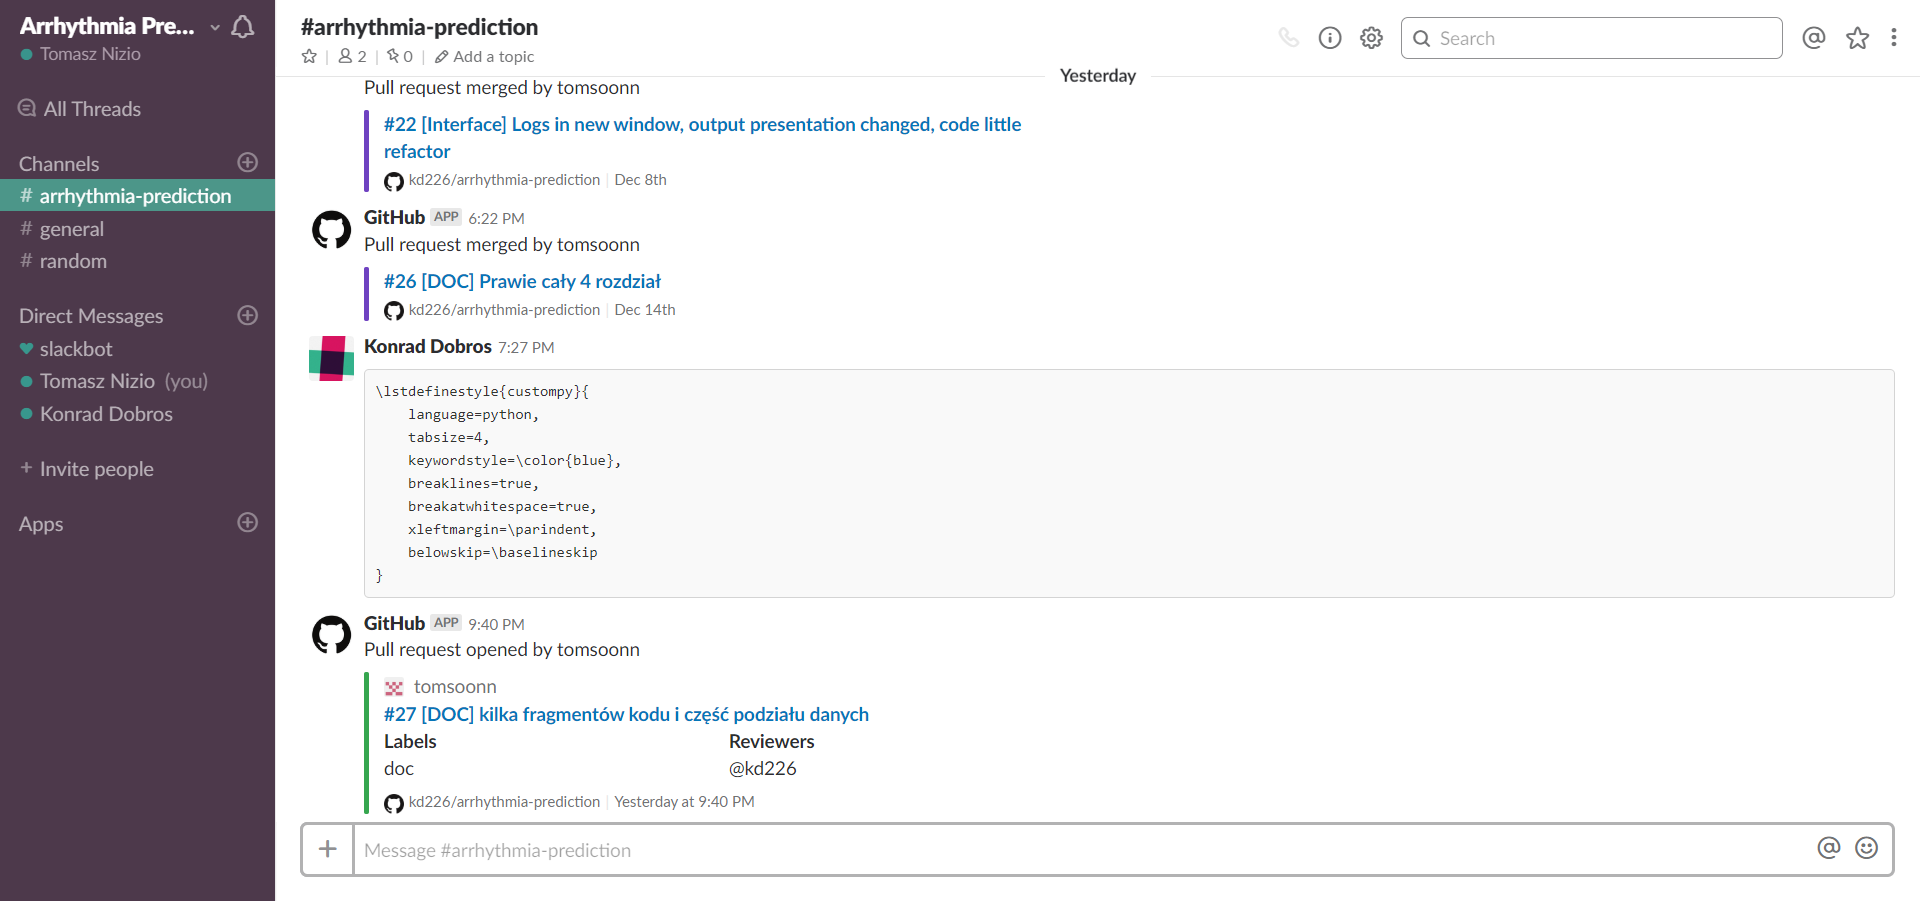
\includegraphics[width=0.9\linewidth]{slack.png}
	\caption{Przykładowy zrzut ekranu z komunikatora Slack}
	\label{fig:slack}
\end{figure}

\begin{figure}[H]
	\centering
	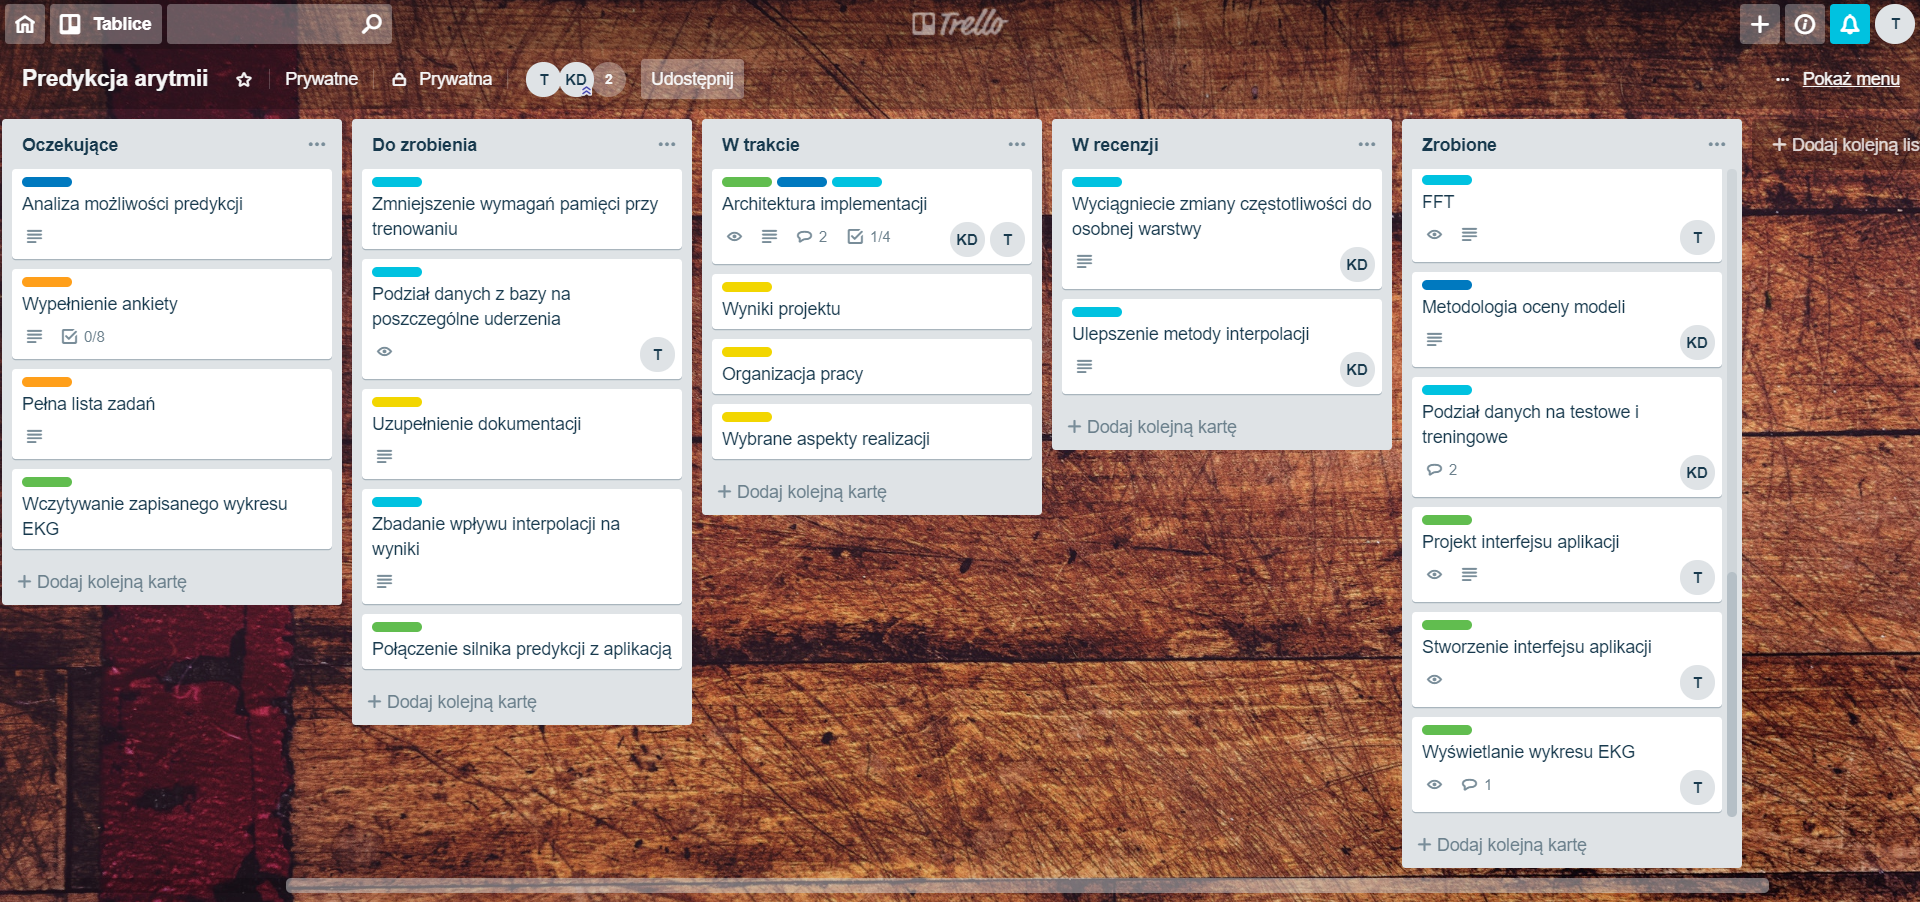
\includegraphics[width=0.9\linewidth]{trello.png}
	\caption{Przykładowy zrzut ekranu z Trello}
	\label{fig:trello}
\end{figure}

Kod wraz z dokumentacją trzymaliśmy w repozytorium \textbf{Git} na platformie \textbf{GitHub}. Do jego tworzenia wykorzystywaliśmy między innymi takie narzędzia jak \textbf{PyCharm} oraz \textbf{JupyterNotebook}, którego pliki zostały zaimportowane do projektu.

Przy tworzeniu interfejsu pomocy był również program \textbf{QtDesigner}.

\begin{figure}[H]
	\centering
	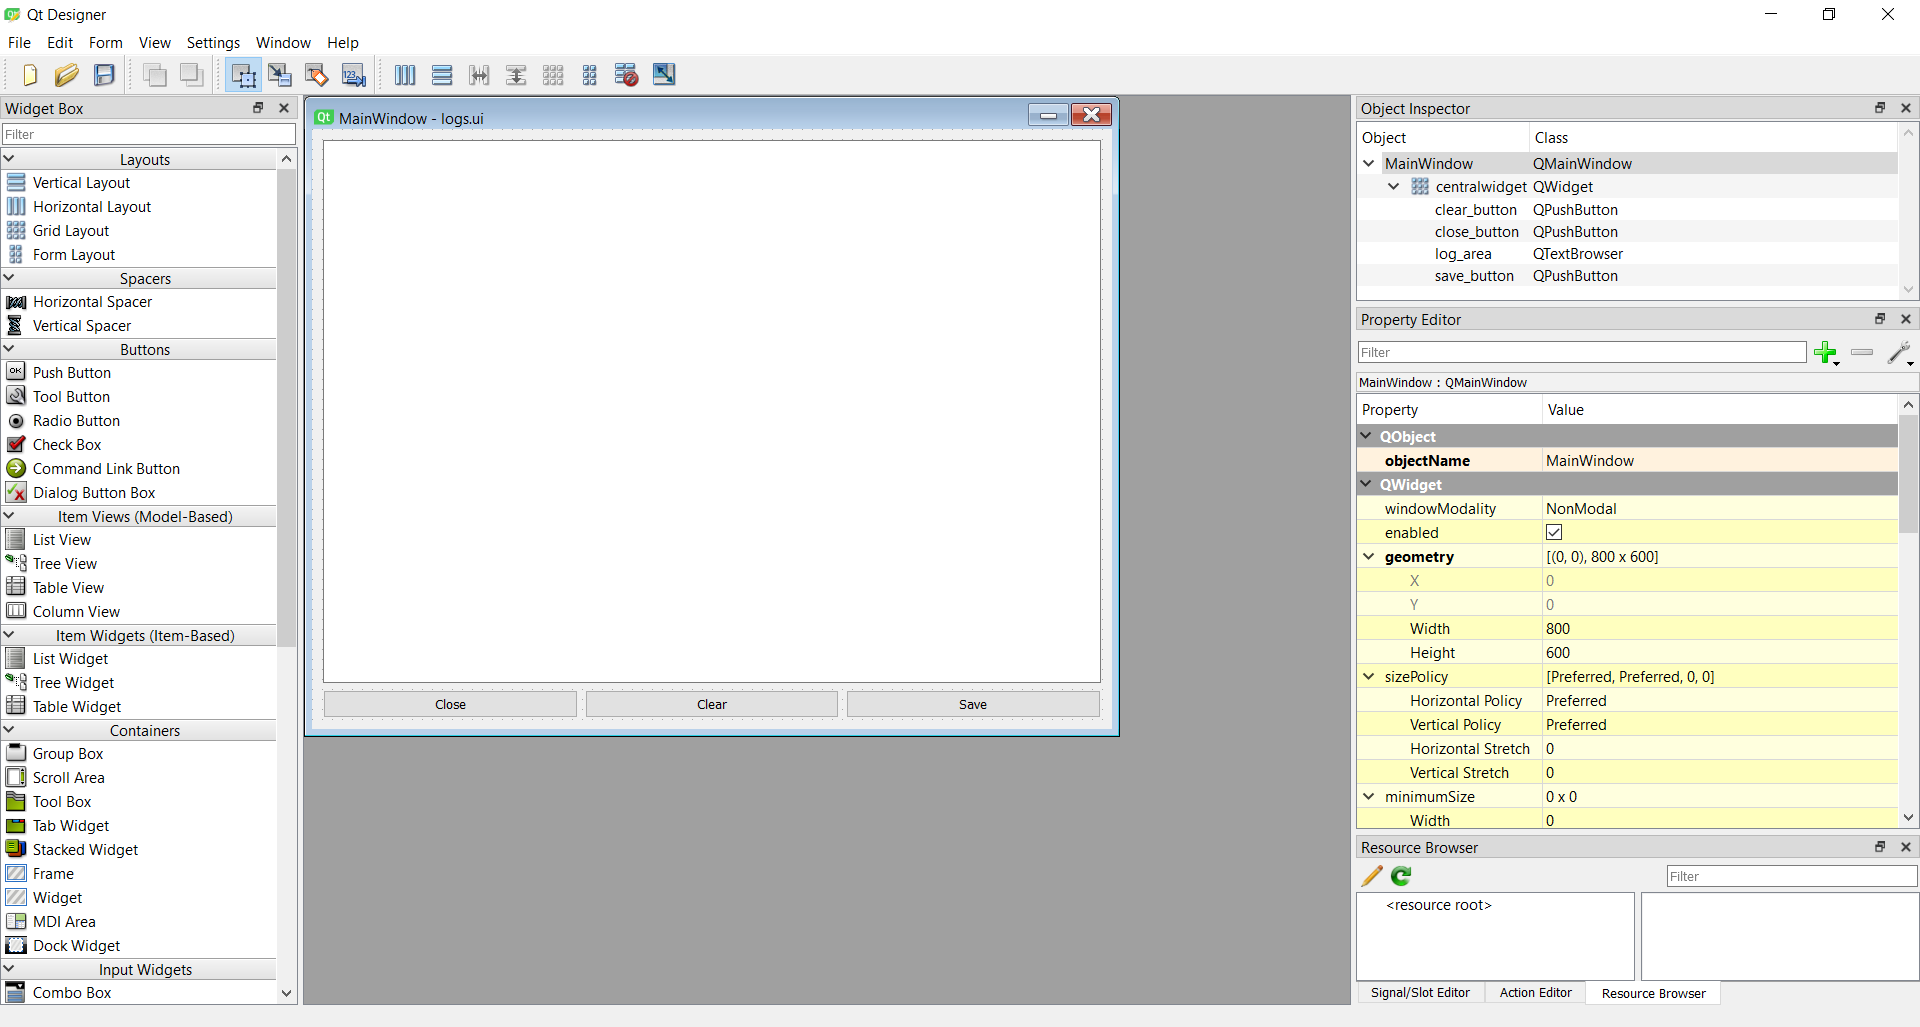
\includegraphics[width=0.8\linewidth]{qt_designer.png}
	\caption{Wygląd programu Qt Designer}
	\label{fig:qt_designer}
\end{figure}

Diagramy rysowaliśmy przy pomocy narzędzia \textbf{draw.io} oraz \textbf{Umlet}.

\section{\SectionTitleResults}
\label{sec:wyniki-projektu}

\subsection{Zrealizowane cele}

Udało nam się zrealizować następujące cele postawione na początku realizacji projektu:
\begin{itemize}
\item wyświetlanie wykresu EKG - wykres jest rysowany
\item możliwość nawigowania po wykresie - możliwe jest przesuwanie wykresu w obydwie strony, a także przeskok do wybranego fragmentu
\item możliwość odtwarzania wykresu EKG - możliwe jest odtwarzanie wykresu dla wczytanych danych co symuluje pracę w czasie rzeczywistym
\item stworzenie oraz przetestowanie skuteczności różnych modeli sieci neuronowych - przetestowane modele zostały opisane w rozdziale 3.3.
\item zintegrowanie ostatecznych modeli z odtwarzaniem wykresu - w trakcie odtwarzania wykresu, co sekundę odbywa się predykcja dla fragmentu EKG kończącego się w tym samym miejscu co aktualnie wyświetlany wykres. Wyniki predykcji wyświetlane są w interfejsie, wpisywane do logów, a także wyświetlany jest wykres jak przebiegała predykcja
\item możliwość przeglądania danych z oznaczonymi typami uderzeń - stworzyliśmy zakładkę na której wykres wyświetlany jest wraz z adnotacjami przy każdym uderzeniu serca 
\item udostępnienie informacji na temat arytmii - stworzyliśmy zakładkę, w której znajduje się lista arytmii wraz z ich opisami
\end{itemize}

\subsection{Najważniejsze wyniki}

%TODO najlepsze wyniki z sieci

\subsection{Wnioski}

%TODO wnioski

\subsection{Możliwości rozwoju}

Projekt można rozbudować o następujące elementy:
\begin{itemize}
\item inne formaty danych - do systemu można dodać obsługę wczytywania danych z plików o innych formatach niż zrealizowane przez nas lub nawet pobieranie danych w czasie rzeczywistym z odpowiednich urządzeń
\item inne typy arytmii - powiększenie bazy uwzględnianych rodzajów uderzeń lub bardziej szczegółowy podział na poszczególne rodzaje
\item nowe modele - poszerzenie listy dostępnych modeli predykcji o nowe modele, być może skuteczniejsze\
\item rysowanie wykresów - optymalizacja rysowania wykresów, zastosowanie grafiki wektorowej
%TODO rozszerzyć
\end{itemize}

\subsection{Podsumowanie}

W ramach tej pracy inżynierskiej udało nam się stworzyć aplikację desktopową spełniającą założone wymagania. Przetestowaliśmy również skuteczność predykcji arytmii przez różne modele predykcji.

Praca nad projektem pozwoliła nam się dużo nauczyć. Przede wszystkim zdobyliśmy cenne doświadczenie pracy w zespole. Nauczyliśmy się sprawnie rozwiązywać problemy pojawiające się w trakcie rozwoju projeku. Poznaliśmy też nowe technologie, które zostały wykorzystane przy tworzeniu systemu.

Jesteśmy zadowoleni z efektu końcowego naszej pracy.



% Tak dla pewności, żeby wypisały się wszystkie materiały, które mamy.
\nocite{*}

\bibliography{bibliografia}

\end{document}
